% \documentclass[conference,compsoc]{IEEEtran}
\documentclass{sig-alternate-05-2015}                

% \usepackage[dvipdfmx]{graphicx} \usepackage{amssymb} \usepackage{multirow} \usepackage{threeparttable} \usepackage{array} \usepackage{color} \usepackage{nidanfloat}
\usepackage{graphicx} \usepackage{amssymb} \usepackage{multirow} \usepackage{threeparttable} \usepackage{array} \usepackage{color} \usepackage{nidanfloat}\usepackage{setspace} 


% \author{\IEEEauthorblockN{Yuya Maruyama}\IEEEauthorblockA{School of Engineering Science\\Osaka University}\and\IEEEauthorblockN{Shinpei Kato}\IEEEauthorblockA{Graduate School of Information Science\\Nagoya University}\and\IEEEauthorblockN{Takuya Azumi}\IEEEauthorblockA{Graduate School of Engineering Science\\Osaka University }}

%% \numberofauthors{3}
%% \author{
%% % 1st. author
%% \alignauthor Yuya Maruyama\\
%% \affaddr{Graduate School of Engineering Science}\\
%% \affaddr{Osaka University}\\
%%        % \affaddr{Institute for Clarity in Documentation}\\
%%        % \affaddr{1932 Wallamaloo Lane}\\
%%        % \affaddr{Wallamaloo, New Zealand}\\
%%        % \email{trovato@corporation.com}
%% % 2nd. author
%% \alignauthor Shinpei Kato\\
%% \affaddr{Graduate School of Information Science and Technology}\\
%% \affaddr{The University of Tokyo}\\
%%        % \affaddr{P.O. Box 1212}\\
%%        % \affaddr{Dublin, Ohio 43017-6221}\\
%%        % \email{webmaster@marysville-ohio.com}
%% % 3rd. author
%% \alignauthor Takuya Azumi\\
%% \affaddr{Graduate School of Engineering Science}\\
%% \affaddr{Osaka University}\\
%% }


% Copyright
\setcopyright{acmcopyright}
%\setcopyright{acmlicensed}
%\setcopyright{rightsretained}
%\setcopyright{usgov}
%\setcopyright{usgovmixed}
%\setcopyright{cagov}
%\setcopyright{cagovmixed}


% DOI
\doi{10.475/123_4}

% ISBN
\isbn{123-4567-24-567/08/06}

%Conference
\conferenceinfo{EMSOFT '16}{October 2--7, 2016, Pittsburgh, PA, USA}

\acmPrice{\$15.00}

%
% --- Author Metadata here ---
% \conferenceinfo{WOODSTOCK}{'97 El Paso, Texas USA}
%\CopyrightYear{2007} % Allows default copyright year (20XX) to be over-ridden - IF NEED BE.
%\crdata{0-12345-67-8/90/01}  % Allows default copyright data (0-89791-88-6/97/05) to be over-ridden - IF NEED BE.
% --- End of Author Metadata ---

\title{Exploring the Performance of ROS2}
\begin{document}

\maketitle

\setcounter{topnumber}{5}%    ページ上部の図表は 5 個まで
\def\topfraction{1.00}%       ページの上 1.00 まで図表で占めて可
\setcounter{bottomnumber}{5}% ページ下部の図表は 5 個まで
\def\bottomfraction{1.00}%    ページの下 1.00 まで図表で占めて可
\setcounter{totalnumber}{10}% ページあたりの図表は 10 個まで
\def\textfraction{0.00}%      ページうち本文が占める割合の下限

% \setlength\textfloatsep{18pt}%  between figure and text
% \setlength\abovecaptionskip{4pt}% between figure and caption
% \setlength\floatsep{18pt}% between figures

\begin{abstract}
  Middleware for robotics development must meet demanding requirements in real-time distributed embedded systems. 
  The Robot Operating System (ROS), open-source middleware, has been widely used for robotics applications.
  However, ROS is not suitable for real-time embedded systems because it does not satisfy real-time requirements and only runs on a few OSs.
  To address this problem, ROS1 will undergo a significant upgrade to ROS2 by utilizing the Data Distribution Service (DDS).
  DDS is suitable for real-time distributed embedded systems due to its various transport configurations (e.g., deadline and fault-tolerance) and scalability.
  ROS2 must convert data for DDS and abstract DDS from its users; however, this incurs additional overhead, which is examined in this study.
  Transport latencies between ROS2 nodes vary depending on the use cases, data size, configurations, and DDS vendors.
  \textcolor{red}{We conduct proof of concept for DDS approach to ROS and arrange DDS characteristic and guidelines from various evaluations.
  By highlighting the DDS capabilities, we explore and evaluate the potential and constraints of DDS and ROS2.}
\end{abstract}

\vspace{-2mm}
\keywords{robot operating system; data distribution service; quality of service; real-time; embedded; publish/subscribe}

\vspace{-3mm}
\section{Introduction}
\label{sec:orgheadline5}

In recent years, real-time distributed embedded systems, such as autonomous driving vehicles, have become increasingly complicated and diverse.
Autonomous driving has attracted attention since the November 3, 2007 DARPA Urban Challenge \cite{urmson2008autonomous}.
The Robot Operating System (ROS) \cite{quigley2009ros} is open-source middleware that has undergone rapid development \cite{cousins2011exponential} and has been widely used for robotics applications (e.g., autonomous driving systems).
The ROS is built almost entirely from scratch and have been maintained by Willow Garage \cite{willowgarage} and Open Source Robotics Foundation (OSRF) \cite{osrf} since 2007. 
The ROS enhances productivity \cite{cousins2010sharing}, providing publish/subscribe transport, multiple libraries (e.g., OpenCV and the Point Cloud Library (PCL) \cite{pcl}), and tools to help software developers create robotics applications.

However, the ROS does not satisfy real-time run requirements and only runs on a few OSs. 
In addition, the ROS cannot guarantee fault-tolerance, deadlines, or process synchronization.
Moreover, the ROS requires significant resources (e.g, CPU, memory, network bandwidth, threads, and cores) and can not manage these resources to meet time constraints.
Thus, the ROS is not suitable for real-time embedded systems. 
This critical problem has been considered by many research communities, including ROS developers, and various solutions have been proposed and evaluated \cite{rosc@roscon2013}, \cite{uros@roscon2013}, \cite{wei2015rt}.
However, these solutions are insufficient\footnote{Reasons why prior work is insufficient are discussed in Section \ref{sec:orgheadline3}.}  to address the ROS's limitations for real-time embedded systems. 

To satisfy the needs of the now-broader ROS community, the ROS will undergo a significant upgrade to ROS2 \cite{ros2_iccps2016}. 
ROS2 will consider the following new use cases: real-time systems, small embedded platforms (e.g., sensor nodes), non-ideal networks, and cross-platform (e.g., Linux, Windows, Mac, Real-Time OS (RTOS), and no OS).
To satisfy the requirements of these new use cases, the existing version of ROS (hereinafter ROS1) will be reconstructed to improve user-interface APIs and incorporate new technologies, such as Data Distribution Service (DDS) \cite{pardo2003omg}, \cite{schlesselman2004omg}, Zeroconf, Protocol Buffers, ZeroMQ, Redis, and WebSockets.\footnote{\textcolor{red}{Currently ROS2 only supports some DDS implementations.}}
The ROS1 transport system will be replaced by DDS, an industry-standard real-time communication system and end-to-end middleware. 
The DDS can provide reliable publish/subscribe transport similar to that of ROS1.

DDS is suitable for real-time embedded systems because of its various transport configurations (e.g., deadline, reliability, and durability) and scalability.
DDS meets the requirements of distributed systems for safety, resilience, scalability, fault-tolerance and security.
DDS can provide solutions for some real-time environments and some small/embedded systems by reducing library sizes and memory footprints.
Developed by different DDS vendors, several implementations of this communication system have been used in mission-critical environments (e.g., trains, aircrafts, ships, dams, and financial systems) and have been verified by NASA and the United States Department of Defense. 
Several DDS implementations have been evaluated and validated by researchers \cite{xiong2010evaluating}, \cite{sierla2003evaluation} and DDS vendors.
These evaluations indicate that DDS is both reliable and flexible.

\textbf{Contribution:}
\textcolor{red}{In this paper, we provide proof of concept for DDS approach to ROS.
We clarify the performance of the data transport for ROS1 and ROS2 in various situations.
Performance means latencies characteristics, throughput and distributed capability.
Focusing on the DDS capabilities, depending on DDS vendor and configuration, we explore and evaluate the potential and constraints from various aspects: latencies, throughput, the number of threads, and memory consumption.
From experimental results, we arrange guidelines and what we can do to solve current constrains.
To the best of our knowledge, this is the first study to explore ROS2 performance.}

\textbf{Organization:} 
The remainder of this paper is organized as follows. 
Section \ref{sec:orgheadline1} provides background information and describes the ROS and DDS system models. 
Section \ref{sec:orgheadline2} validates experimental situations and evaluates the performance of ROS1 and ROS2 with various configurations. 
Section \ref{sec:orgheadline3} discusses related work. 
Finally, Section \ref{sec:orgheadline4} concludes the paper and offers suggestions for future work.

\vspace{-3mm}
\section{Background}
\label{sec:orgheadline1}

In this section, we provide background knowledge. 
First, we describe the ROS2 system model compared to ROS1, focusing on its communication system. 
We then review aspects of the ROS, such as the publish/subscribe model. 
Finally, we describe DDS, which is used as the communication system for real-time systems in ROS2. 

\vspace{-1mm}
\subsection{Robot Operating System (ROS)}
\label{sec:orgheadline6}

\begin{figure}[t]
  \centering
  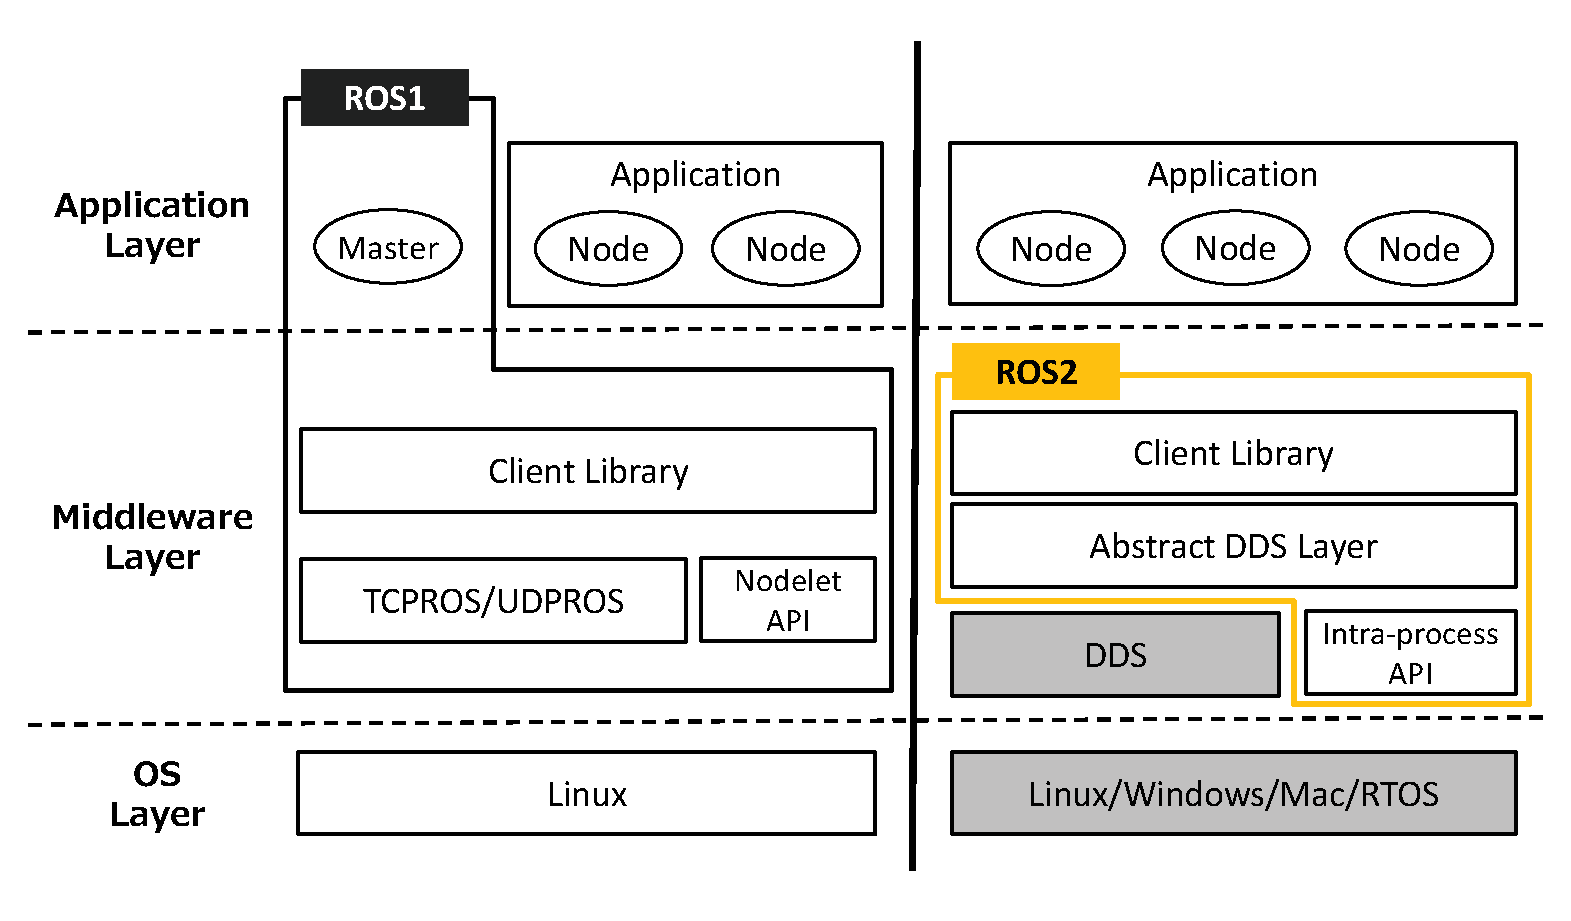
\includegraphics[width=0.9\linewidth]{../figure/ros_architecture.eps}
  \vspace{-5mm}
  \caption{\label{fig:orgparagraph1}
    ROS1/ROS2 architecture.}
  \vspace{-6mm}
\end{figure}   

Figure \ref{fig:orgparagraph1} briefly illustrates the system models of ROS1 and ROS2. 
In the left side of Figure \ref{fig:orgparagraph1}, ROS1's implementation includes the communication system, TCPROS/UDPROS.
This communication requires a master process (unique in the distributed system) because of the implementation of ROS1.
In contrast, as shown in the right side of Figure \ref{fig:orgparagraph1}, ROS2 builds upon DDS and contains a DDS abstraction layer. 
Users do not need to be aware of the DDS APIs due to this abstraction layer.
This layer allows ROS2 to have high-level configuration and optimizes the utilization of DDS. 
In addition, due to use of DDS, ROS2 does not need a master process.
\textcolor{red}{This is a import point in terms of fault tolerance.}

ROS applications consist of independent computing processes called \emph{nodes}, which promote fault isolation, faster development, modularity, and code reusability. 
Communication among \emph{nodes} is based on a publish/subscribe model. 
In this model, \emph{nodes} communicate by passing \emph{messages} via a \emph{topic}. 
A \emph{message} has a simple data structure (much like C structs) defined by .msg files.
\emph{Nodes} identify the content of the \emph{message} by the \emph{topic} name.
As a \emph{node} publishes a \emph{message} to a \emph{topic}, another \emph{node} subscribes to the \emph{topic} and utilizes the \emph{message}. 
For example, as shown in Figure \ref{fig:orgparagraph2}, the ``Camera'' \emph{node} sends \emph{messages} to the ``Images'' \emph{topic}. 
The \emph{messages} in the \emph{topic} are received by the ``Car Detection'' \emph{node}  and ``Pedestrian Detection'' \emph{node}.
The publish/subscribe model is designed to be modular at a fine-grained scale and is suitable for distributed systems.

\begin{figure}[t]
  \centering
  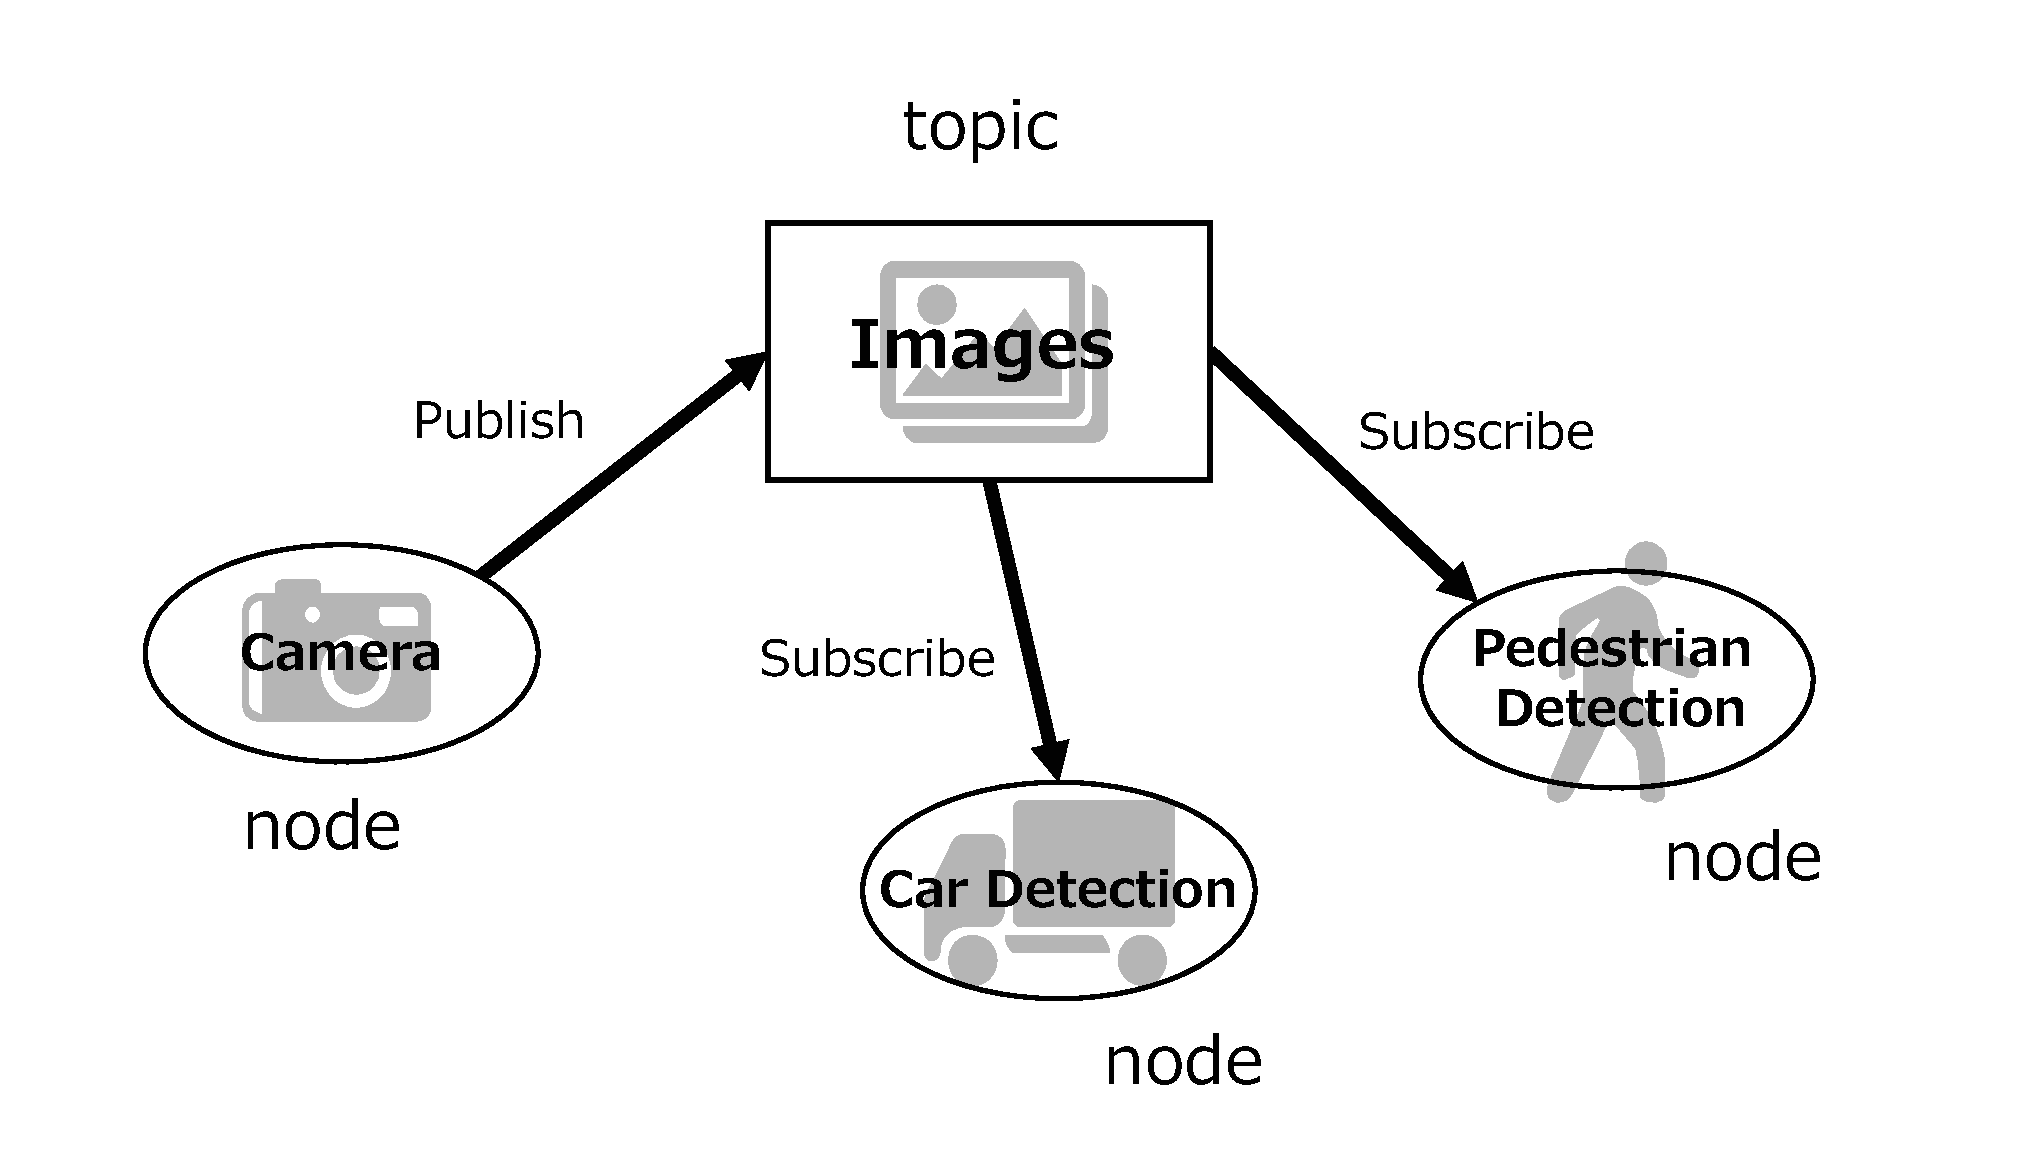
\includegraphics[width=0.8\linewidth]{../figure/ros_pubsub_fig.eps}
  \vspace{-5mm}
  \caption{\label{fig:orgparagraph2}
    Example of ROS publish/subscribe model.}
  \vspace{-6mm}
\end{figure}

In ROS1, the above communication system is implemented as middleware based on TCPROS and UDPROS using TCP/IP and UDP/IP sockets. 
When \emph{subscriber-nodes} and \emph{publisher-nodes} are launched, they interact with a \emph{master-node} that collects information and manages all \emph{topics}, similar to a server. 
After an XML/Remote Procedure Call (RPC) transaction with the \emph{master-node}, \emph{subscriber-nodes} request a connection to \emph{publisher-nodes}, using an agreed upon connection protocol. 
Actual data (i.e., a \emph{message}) is transported directly between \emph{nodes}. 
Data does not route through the master. 
ROS1 realizes a peer-to-peer data transport between \emph{nodes}. 

Optionally, ROS1 provides \emph{nodelets}, which provide efficient \emph{node} composition for optimized data transport without TCPROS and UDPROS. 
A \emph{nodelet} realizes non-serialized data transport between \emph{nodes} in the same process by passing a pointer. 
ROS2 inherits this option as \emph{intra-process communication}, which addresses some of the fundamental problems with \emph{nodelets} (e.g., safe memory access).

ROS2 adopts DDS as its communication system. However, as an exception, \emph{intra-process communication} is executed without DDS.
DDS is provided by many vendors and has several implementation types.
Developers can select appropriate DDS implementations from a variety of DDS vendors.

\vspace{-1mm}
\subsection{Data Distribution Service (DDS)}
\label{sec:orgheadline7}

The DDS specification \cite{dds1.4} is defined for a publish/subscribe data-distribution system by the Object Management Group (OMG) \cite{omg}. 
The OMG manages the definitions and standardized APIs; however the OMG hides the details of implementation. Several implementations have been developed by different vendors (e.g., RTI \cite{rti_connext} and PRISMTECH \cite{ospl_dds_community}).
DDS supports a wide range of applications, from small embedded systems to large scale systems, such as infrastructures. 
Note that distributed real-time embedded systems are also supported.

The core of DDS is a Data-Centric Publish-Subscribe (DCPS) model designed to provide efficient data transport between processes even in distributed heterogeneous platforms. 
The DCPS model creates a ``global data space'' that can be accessed by any independent applications. 
DCPS facilitates efficient data distribution.
In DDS, each process that publishes or subscribes to data is called a \emph{participant}, which corresponds to a \emph{node} in the ROS. 
\emph{Participants} can read and write from/to the global data space using a typed interface.

As shown in Figure \ref{fig:orgparagraph3}, the DCPS model is constructed of \emph{DCPS Entities}: \emph{DomainParticipant}, \emph{Publisher}, \emph{Subscriber}, \emph{DataWriter}, \emph{DataReader}, and \emph{Topic}. 
Each data transport between processes is executed according to a \emph{Quality of Service (QoS) Policy}.

\begin{figure}[t]
  \centering
  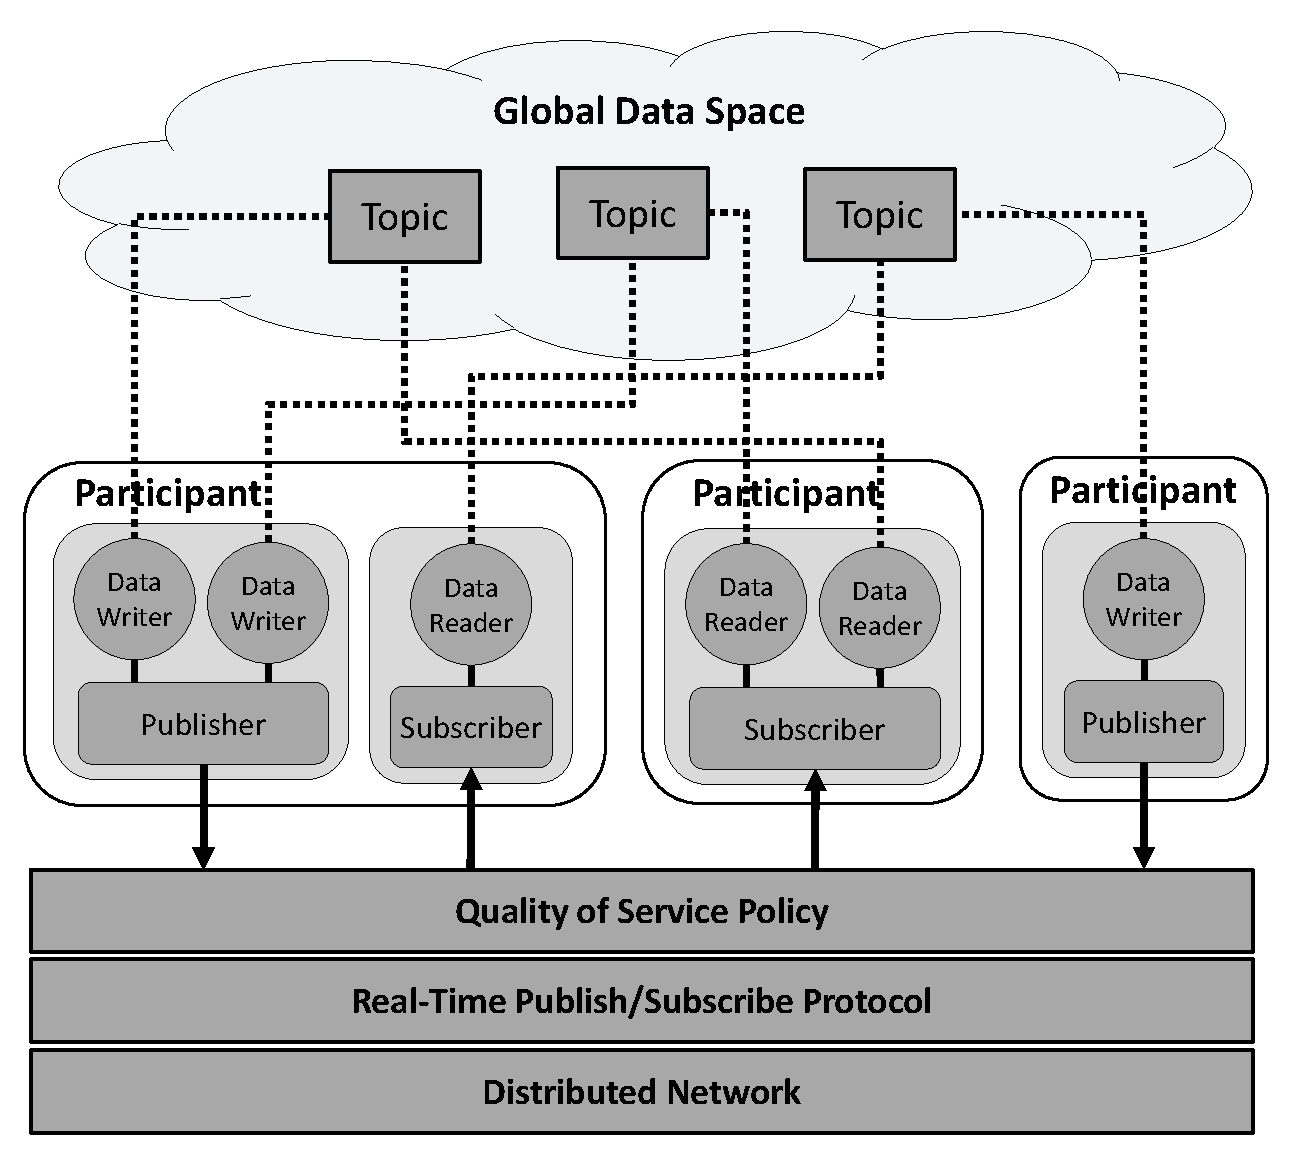
\includegraphics[width=0.7\linewidth]{../figure/DDS_model.eps}
  \vspace{-3mm}
  \caption{\label{fig:orgparagraph3}
    Data-centric publish-subscribe (DCPS) model.}
  \vspace{-5mm}
\end{figure}   

\noindent \textbf{\emph{DomainParticipant}:} 
A \emph{DomainParticipant} is a container for following other entities and the entry-point for the service. 
In DDS, all applications communicate with each other within a \emph{Domain}, which promotes isolation and communication optimization.

\noindent \textbf{\emph{Publisher}:} 
A \emph{Publisher} is the object responsible for data issuance. 
Managing one or several \emph{DataWriters}, the \emph{Publisher} sends data to one or more \emph{Topics}.

\noindent \textbf{\emph{Subscriber}:} 
A \emph{Subscriber} is responsible for receiving published data and making the data available. 
The \emph{Subscriber} acts on behalf of one or more \emph{DataReaders}. 
According to a \emph{Subscriber}, a \emph{DomainParticipant} can receive and dispatch data of different specified types.

\noindent \textbf{\emph{DataWriter}:} 
A \emph{DataWriter} is an object that must be used by a \emph{DomainParticipant} to publish data through a \emph{Publisher}. 
The \emph{DataWriter} publishes data of a given type.

\noindent \textbf{\emph{DataReader}:} 
A \emph{DataReader} is an object that is attached to a \emph{Subscriber}. 
Using the \emph{DataReader}, a \emph{DomainParticipant} can receive and access data whose type must correspond to that of the \emph{DataWriter}.

\noindent \textbf{\emph{Topic}:} 
A \emph{Topic} is used to identify each data-object between a \emph{DataWriter} and a  \emph{DataReader}. 
Each \emph{Topic} is defined by a name and a data type. 

\noindent \textbf{\emph{QoS Policy}:} 
All \emph{DCPS Entities} have a \emph{QoS Policy}, which represents their data transport behavior. 
Each data transaction is configurable at various levels of granularity via many \emph{QoS Policy} options. 
In Figure \ref{fig:orgparagraph4}, we show an example of DDS data transport following a \emph{QoS Policy}. 
The deadline period, depth of history, and communication reliability are configured by a \emph{QoS Policy}. 
Table \ref{tab:orgtable1} shows the details of the \emph{QoS Policy} supported by ROS2. 
In DDS, there are many other \emph{QoS Policies} \cite{dds1.4}, which ROS2 should support to extend its capabilities.

\begin{figure}[t]
  \centering
  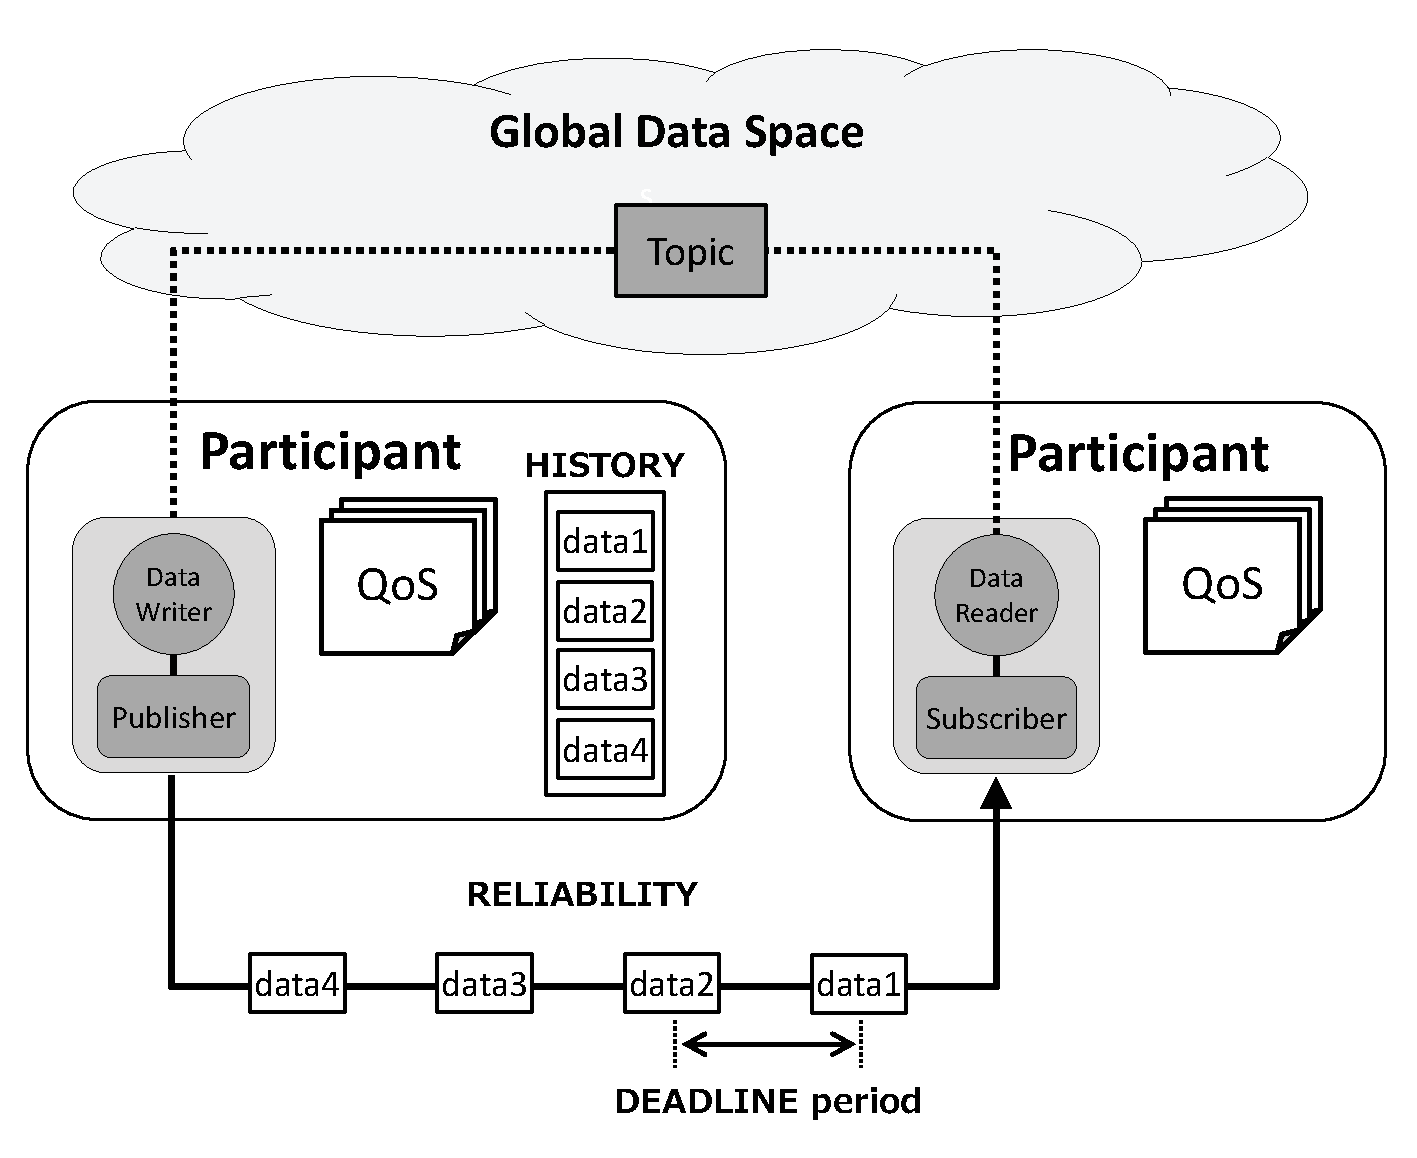
\includegraphics[width=0.8\linewidth]{../figure/DDS_qos.eps}
  \vspace{-3mm}
  \caption{\label{fig:orgparagraph4}
    DDS QoS Policy.}
  \vspace{-5mm}
\end{figure}

\renewcommand{\arraystretch}{1.0}
\begin{table}[t]
  \caption{\label{tab:orgtable1}
    All QoS Policies of ROS2}
  \centering
  \small
  \tabcolsep = 0.5mm              % side-margin in column
  \begin{tabular}{|p{0.23\linewidth}|p{0.74\linewidth}|}
    \hline
    DEADLINE &  A \emph{DataWriter} and a \emph{DataReader} must update data at least once every deadline period.\\
    \hline
    HISTORY &  This controls whether the data transport should deliver only the most recent value, attempt to deliver all intermediate values, or attempt to deliver something in between (configurable via the \texttt{depth} option).\\
    \hline
    RELIABILITY & In \texttt{BEST\_EFFORT}, data transport is executed as soon as possible. However, some data may be lost if the network is not robust. \\
    & In \texttt{RELIABLE}, missed samples are retransmitted. Therefore, data delivery is guaranteed.\\
    \hline
    DURABILITY & With this policy, the service attempts to keep several samples so that they can be delivered to any potential late-joining \emph{DataReader}. The number of saved samples depends on HISTORY. This option has several values, such as \texttt{VOLATILE} and \texttt{TRANSIENT\_LOCAL}.\\
    \hline
  \end{tabular}
  \vspace{-7mm}
\end{table}

In the DCPS model, data of a given type is published from one or several \emph{DataWriters} to a \emph{topic} (its name is unique in the \emph{Domain}).
One or more \emph{DataReaders} identify a data-object by \emph{topic} name in order to subscribe to the \emph{topic}. 
After this transaction, a \emph{DataWriter} connects to a \emph{DataReader} using the Real-Time Publish/Subscribe (RTPS) protocol \cite{rtps2.2} in distributed systems. 
The RTPS protocol, the DDS standard protocol, allows DDS implementations from multiple vendors to inter-operate by abstracting and optimizing transport, such as TCP/UDP/IP. 
The RTPS protocol is flexible and is defined to take advantage of a \emph{QoS Policy}. 
Several vendors use UDP and shared memory transport to communicate. 
However, in several circumstances, the TCP protocol might be required for discovery and data exchange.

Data transport between a \emph{DataWriter} and a \emph{DataReader} is executed in the RTPS protocol according to a \emph{QoS Policy}. 
Each \emph{DCPS Entity} manages data samples according to a unique user-specified \emph{QoS Policy}. 
The DCPS middleware is responsible for data transport in distributed systems based on the \emph{QoS Policy}. 
Without considering detailed transport implementations, DDS users generate code as a \emph{DomainParticipant}, including \emph{QoS Policies} using the DDS APIs. 
Thus, users can focus solely on their purpose and determine ways to satisfy real-time constraints easily. 

\vspace{-3mm}
\section{Evaluations}
\label{sec:orgheadline2}

This section clarifies the capabilities and latencies characteristics of ROS1 and ROS2. 
At present, ROS2 has been released as an alpha version whose major features are a C++ client library, a build-system and abstraction to a part of the DDS middleware from several vendors. 
Note that ROS2 is a very rough draft and is currently under heavy development. 
Therefore, this evaluation attempts to clarify the currently achievable capabilities and latencies characteristics of ROS2.

The following experiments were conducted to evaluate end-to-end latencies for publish/subscribe messaging. 
The latencies are measured from a publish function on a single \emph{node} until the callback function of another \emph{node} using the hardware and software environment listed in Table \ref{tb:environment}. 
The range of the transferred data size is 256 B to 4 MB because large image data (e.g., 2 MB) and point cloud data (.pcd) are frequently used in ROS applications, such as an autonomous driving system \cite{kato2015open}.
A string type \emph{message} is used for this evaluation.
In the following experiments, we use two QoS settings, i.e.,  \texttt{reliable policy} and \texttt{best-effort policy}, as shown in Table \ref{tab:orgtable2}. 
In the \texttt{reliable policy}, \texttt{TRANSIENT\_LOCAL} allows a \emph{node} to keep all \emph{messages} for late-joining \emph{subscriber-nodes}, and \texttt{RELIABLE} facilitates reliable communication.
In the \texttt{best-effort policy}, \emph{nodes} do not keep \emph{messages} and communicate unreliably.
While each \emph{node} is executed at 10 Hz, the experiments are repeated up to 4 MB. Boxplots and the medians obtained from 100 measurements for each data size are presented.
\textcolor{red}{For precise evaluation methods, we make the source code open in \cite{m_yuya_ros1} and \cite{m_yuya_ros2}.}
We compare three DDS implementations, i.e., Connext \cite{rti_connext}, OpenSplice \cite{ospl_dds_community}, and FastRTPS \cite{fastrtps}. 
Connext and OpenSplice are well-known commercial license DDS implementations. 
Note that Connext also has a research license. 
Several implementations of OpenSplice and FastRTPS have been released under the LGPL license. 
By default, Connext uses UDPv4 and shared memory to exchange data. 
Note that OpenSplice\footnote{Vortex OpenSplice \cite{ospl_vortex}, i.e., OpenSplice commercial edition, supports shared memory transport\textcolor{red}{, but ROS2 does not support this.} In this paper, OpenSplice DDS Community Edition is used because it is open-source.} 
and FastRTPS do not support shared memory data transport. 
For precise evaluations and real-time requirements, \emph{nodes} follow \emph{SCHED\_FIFO} \cite{garg2009real} and the \emph{mlockall} system call. 
A \emph{SCHED\_FIFO} process preempts any non-\emph{SCHED\_FIFO} processes, i.e., processes that use the default Linux scheduling.
Using \emph{mlockall}, a process's virtual address space is fixed in physical RAM, thereby preventing that memory from being paged to the swap area.

\begin{table}[t]
  \caption{Evaluation Environment} 
  \vspace{-3mm}
  \centering
  \begin{threeparttable}
    \renewcommand{\arraystretch}{1.0}
    \label{tb:environment}
    \small
    \tabcolsep = 1.5mm              % side-margin in column
    \begin{tabular}{c|c||c|c}
      \hline
      \multicolumn{2}{c||}{ } & \textbf{\texttt{Machine1}} & \textbf{\texttt{Machine2}} \\ \hline \hline
      \multirow{4}{*}{CPU}   & Model number & Intel Core i5 3470 & Intel Core i5 2320 \\ 
      & Frequency & 3.2 GHz & 3.00 GHz \\ 
      & Cores & 4 & 4 \\ 
      & Threads & 4 & 4 \\ \hline
      \multicolumn{2}{c||}{Memory} & 16 GB & 8 GB \\ \hline 
      \multicolumn{2}{c||}{\textcolor{red}{Network}} & \multicolumn{2}{c}{\textcolor{red}{100 Mbps Ethernet / Full-Duplex}} \\ \hline
      \multicolumn{2}{c||}{ROS1} & \multicolumn{2}{c}{Indigo} \\ 
      \multicolumn{2}{c||}{ROS2} & \multicolumn{2}{c}{Cement (alpha3)} \\ 
      \multicolumn{2}{c||}{DDS implementations} & \multicolumn{2}{c}{Connext\tnote{1} / OpenSplice\tnote{2} / FastRTPS } \\ \hline 
      \multirow{2}{*}{OS} & Distribution & \multicolumn{2}{c}{Ubuntu 14.04} \\ 
      & Kernel & \multicolumn{2}{c}{Linux 3.13.0} \\ \hline
    \end{tabular}
    \begin{tablenotes}
    \item[1] RTI Connext DDS Professional \cite{rti_connext}
    \item[2] OpenSplice DDS Community Edition \cite{ospl_dds_community}
    \end{tablenotes}
  \end{threeparttable}
  \vspace{-5mm}
\end{table}

\renewcommand{\arraystretch}{1.0}
\begin{table}[t]
  \caption{\label{tab:orgtable2}
    QoS Policies for Evaluations}
  \centering
  \tabcolsep = 1.5mm              % side-margin in column
  \begin{tabular}{c|cc}
    \hline
    & \textbf{\texttt{reliable policy}} & \textbf{\texttt{best-effort policy}}\\
    \hline
    \hline
    DEADLINE & \texttt{100 ms} & \texttt{100 ms}\\
    HISTORY & \texttt{ALL} & \texttt{LAST}\\
    depth & \texttt{-} & \texttt{1}\\
    RELIABILITY & \texttt{RELIABLE} & \texttt{BEST\_EFFORT}\\
    DURABILITY & \texttt{TRANSIENT\_LOCAL} & \texttt{VOLATILE}\\
    \hline
  \end{tabular}
  \vspace{-5mm}
\end{table}

\newcommand*{\x}[0]{\checkmark} % set macro
\newcommand*{\y}[1]{$\blacktriangle^{#1}$} % set macro (ex. \y{1} or \z1 )
\newcommand*{\z}[1]{$\triangle^{#1}$} % set macro 

\begin{table*}[t]
  \renewcommand{\arraystretch}{1.1}
  \caption{Capabilities of ROS1 and/or ROS2 for each Data Transport} 
  \label{tb:capabilities}
  \centering
  \tabcolsep = 1.4mm              % side-margin in column
  \small
  \scalebox{0.85}{
    % \begin{tabular}{c|c|c|c||c|c*{11}{>{\centering\arraybackslash}p{4mm}}}
    \begin{tabular}{c|c|c|c||c|c*{11}{c}}
      \hline
      \multicolumn{4}{c||}{ } & \textbf{Initial loss} & \textbf{256 [byte]} & \textbf{512} & \textbf{1K} & $\cdots$
      $^{*}$
      & \textbf{64K} & \textbf{128K}  & \textbf{256K} & \textbf{512K} & \textbf{1M} & \textbf{2M} & \textbf{4M}\\ \hline \hline
      \multirow{3}{*}{ROS1}   & \multicolumn{3}{c||}{(1-a) remote}  &any&\x&\x&\x&$\cdots$&\x&\x&\x&\x&\x&\z1&\z1&\\ \cline{2-4}
      & \multicolumn{3}{c||}{(1-b) local}  &any&\x&\x&\x&$\cdots$&&\x&\x&\x&\x&\x&\x&\\ \cline{2-4}
      & \multicolumn{3}{c||}{(1-c) nodelet}  &none&\x&\x&\x&$\cdots$&\x&\x&\x&\x&\x&\x&\x&\\ \hline
      \multirow{11}{*}{ROS2}  & \multirow{5}{*}{(2-a) remote}  & \multirow{2}{*}{Connext}  & reliable &none&\x&\x&\x&$\cdots$&\x&\y2&\y2&\y2&\y2&\y2&\y2&\\ \cline{4-4}
      & & & best-effort &none&\x&\x&\x&$\cdots$&\x&\x&\x&\x&\x&\z1&\z1&\\ \cline{3-4}
      & & \multirow{2}{*}{OpenSplice}  & reliable &none&\x&\x&\x&$\cdots$&\x&\x&\x&\x&\x&\x&\x&\\ \cline{4-4}
      & & & best-effort &none&\x&\x&\x&$\cdots$&\x&\x&\x&\x&\x&\z1&\z1&\\ \cline{3-4}
      & & \multicolumn{2}{c||}{FastRTPS} &none&\y3&\y3&\y3&$\cdots$&\y3&\y3&\y3&\y3&\y3&\y3&\y3&\\ \cline{2-4} 
      & \multirow{5}{*}{(2-b) local}  & \multirow{2}{*}{Connext}  & reliable &none&\x&\x&\x&$\cdots$&\x&\y2&\y2&\y2&\y2&\y2&\y2&\\ \cline{4-4}
      & & & best-effort &none&\x&\x&\x&$\cdots$&\x&\x&\x&\x&\x&\z2&\y1&\\ \cline{3-4}
      & & \multirow{2}{*}{OpenSplice}  & reliable &none&\x&\x&\x&$\cdots$&\x&\x&\x&\x&\x&\x&\x&\\ \cline{4-4}
      & & & best-effort &none&\x&\x&\x&$\cdots$&\x&\x&\x&\x&\x&\z2&\z2&\\ \cline{3-4}
      & & \multicolumn{2}{c||}{FastRTPS} &none&\y3&\y3&\y3&$\cdots$&\y3&\y3&\y3&\y3&\y3&\y3&\y3&\\ \cline{2-4} 
      & \multicolumn{3}{c||}{(2-c) intra-process} &none&\x&\x&\x&$\cdots$&\x&\x&\x&\x&\x&\x&\x&\\ \hline
      \multirow{4}{*}{ROS1 to 2} & \multirow{2}{*}{(3-a) remote} & \multicolumn{2}{c||}{Connext} &any&\x&\x&\x&$\cdots$&\x&\x&\x&\x&\x&\y1&\y1&\\ \cline{3-4}
      & & \multicolumn{2}{c||}{OpenSplice} &any&\x&\x&\x&$\cdots$&\x&\x&\x&\x&\x&\z1&\z1&\\ \cline{2-4}
      & \multirow{2}{*}{(3-b) local} & \multicolumn{2}{c||}{Connext} &any&\x&\x&\x&$\cdots$&\x&\x&\x&\x&\x&\y1&\y1&\\ \cline{3-4}
      & & \multicolumn{2}{c||}{OpenSplice} &any&\x&\x&\x&$\cdots$&\x&\x&\x&\x&\x&\x&\x&\\ \hline
      \multirow{4}{*}{ROS2 to 1} & \multirow{2}{*}{(3-a) remote} & \multicolumn{2}{c||}{Connext} &any&\x&\x&\x&$\cdots$&\x&\x&\x&\x&\x&\y1&\y1&\\ \cline{3-4}
      & & \multicolumn{2}{c||}{OpenSplice} &any&\x&\x&\x&$\cdots$&\x&\x&\y1&\y1&\y1&\y1&\y1&\\ \cline{2-4}
      & \multirow{2}{*}{(3-b) local} & \multicolumn{2}{c||}{Connext} &any&\x&\x&\x&$\cdots$&\x&\x&\x&\x&\x&\y1&\y1&\\ \cline{3-4}
      & & \multicolumn{2}{c||}{OpenSplice} &any &\x&\x&\x&$\cdots$&\x&\x&\z1&\y1&\y1&\y1&\y1&\\ \hline
    \end{tabular}
  }
  \\ 
  \vspace{-3mm}
  \begin{flushleft}
    $^{*}$: same behavior as 1 and 64 KB;
    \x : data transport possible;   
    \z1: possible but missing the deadline;   
    \z2: data loss possible; \\
    \y1: impossible due to a halt of process or too much data loss; \\
    \y2: impossible with an error message (deficiency of additional configurations for large data); \\
    \y3: impossible with an error message (unsupported large data for the DDS implementation) \\
  \end{flushleft}
  \vspace{-8mm}
\end{table*}


\vspace{-1mm}
\subsection{Experimental Situations and Methods}
\label{sec:orgheadline8}

\begin{figure}[t]
  \centering
  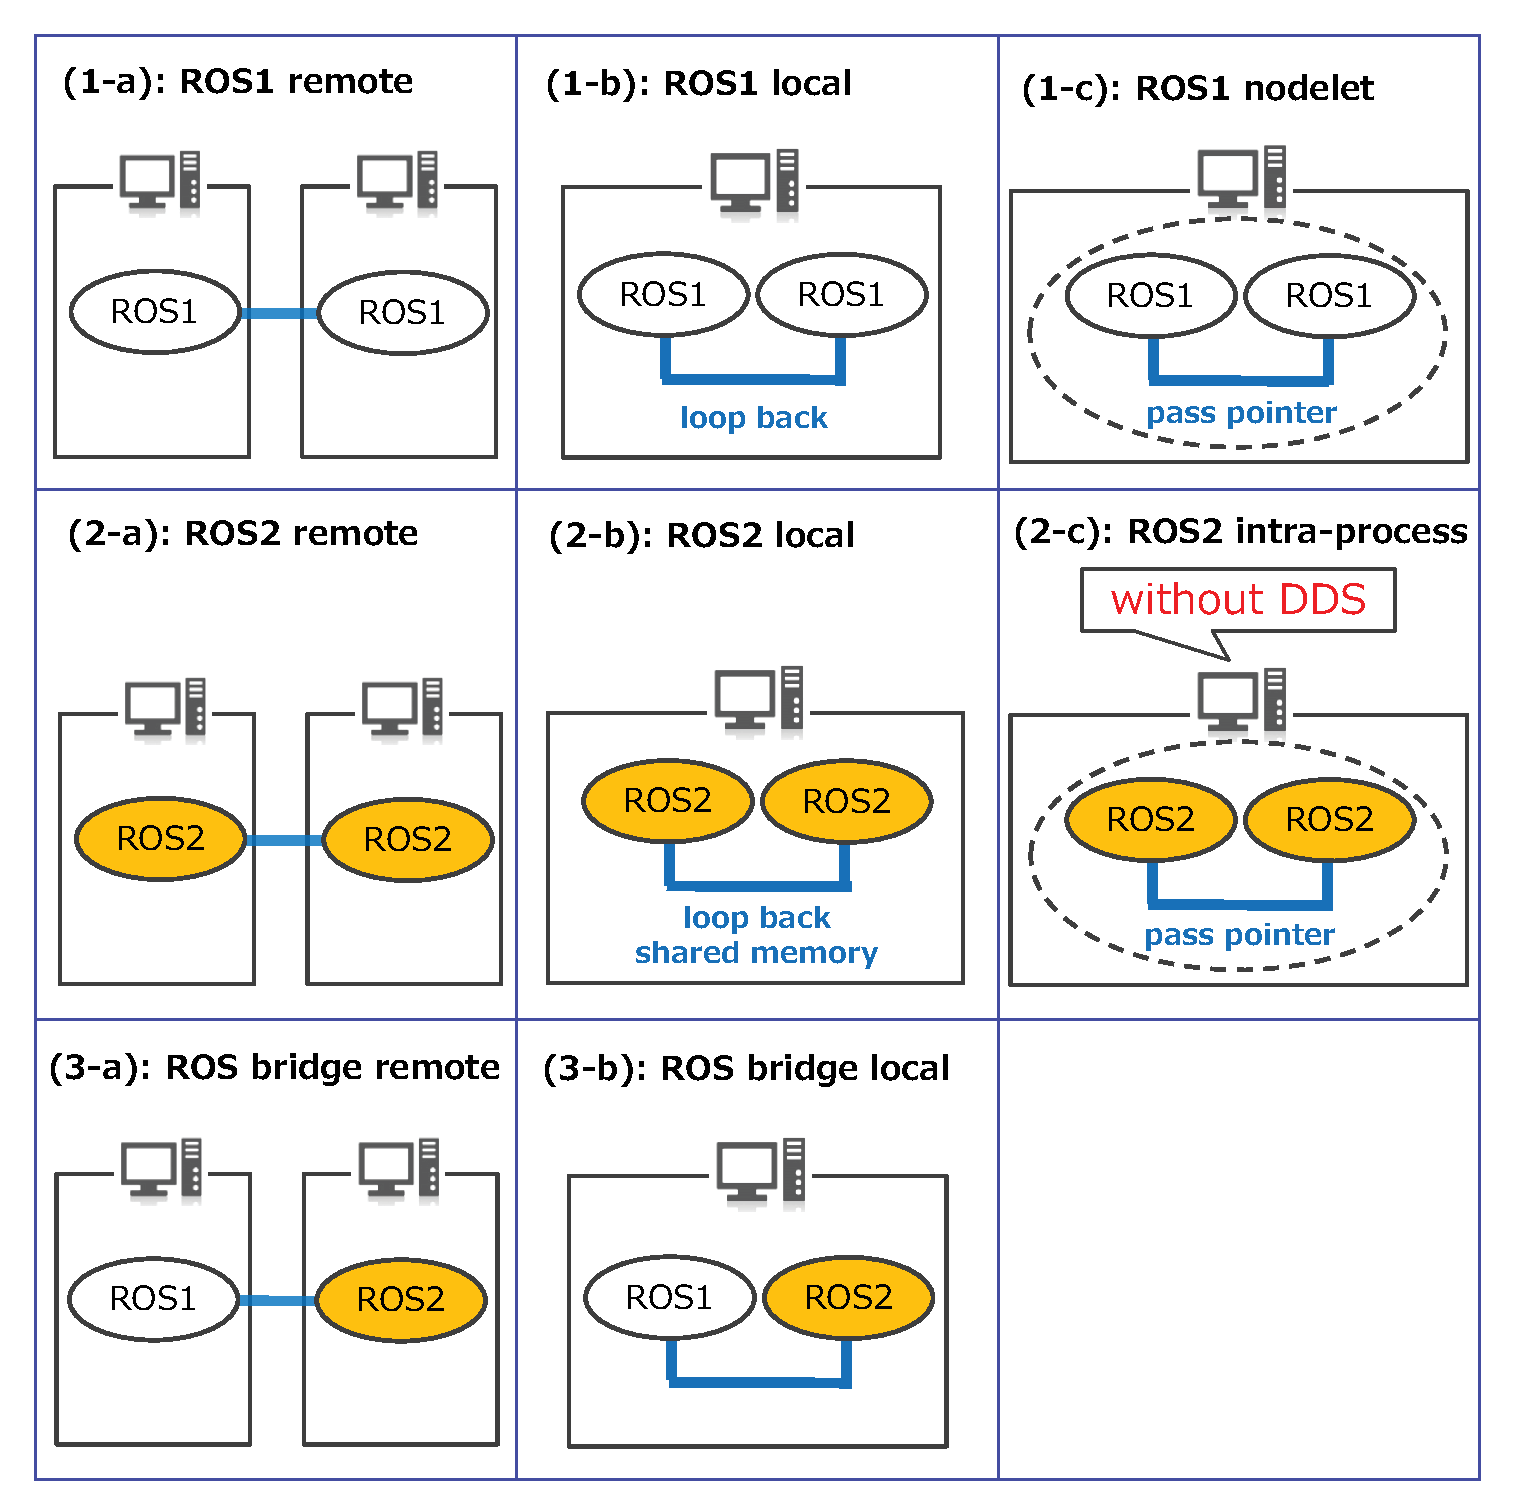
\includegraphics[width=0.8\linewidth]{../figure/eval_situation.eps}
  \vspace{-4mm}
  \caption{\label{fig:orgparagraph5}
    Experimental situations.}
  \vspace{-3mm}
\end{figure}

\begin{figure}[t]
  \centering
  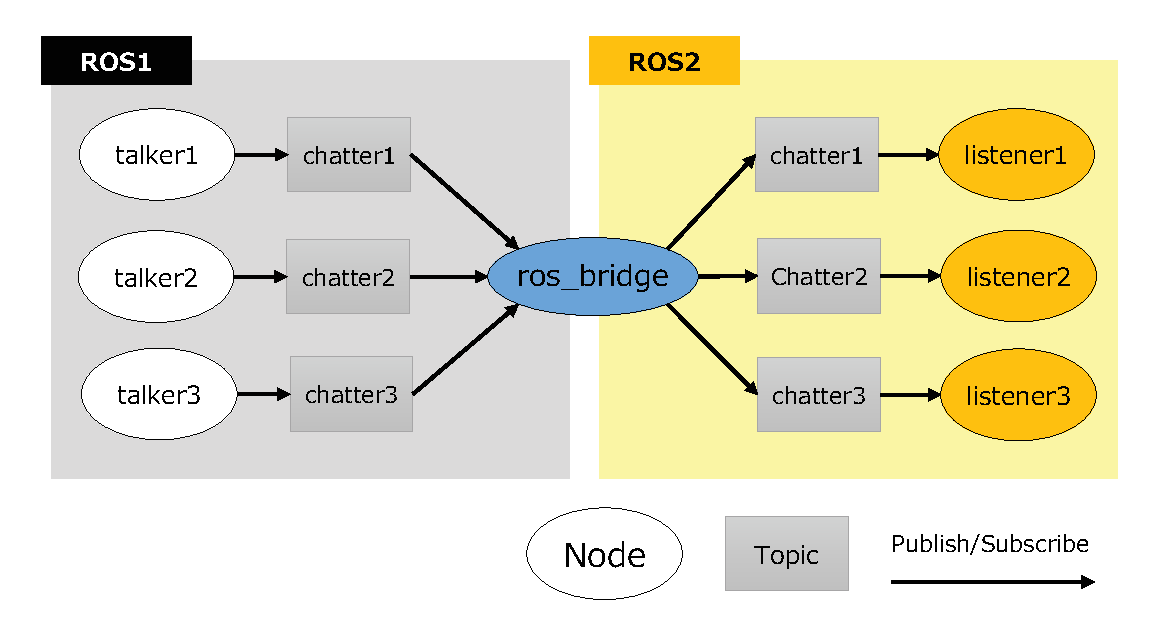
\includegraphics[width=0.9\linewidth]{../figure/ros_bridge.eps}
  \vspace{-8mm}
  \caption{\label{fig:orgparagraph6}
    \texttt{ros\_bridge} evaluation in (3-a) and (3-b).}
  \vspace{-6mm}
\end{figure}

%% \begin{figure*}[t]
%% \centering
%% 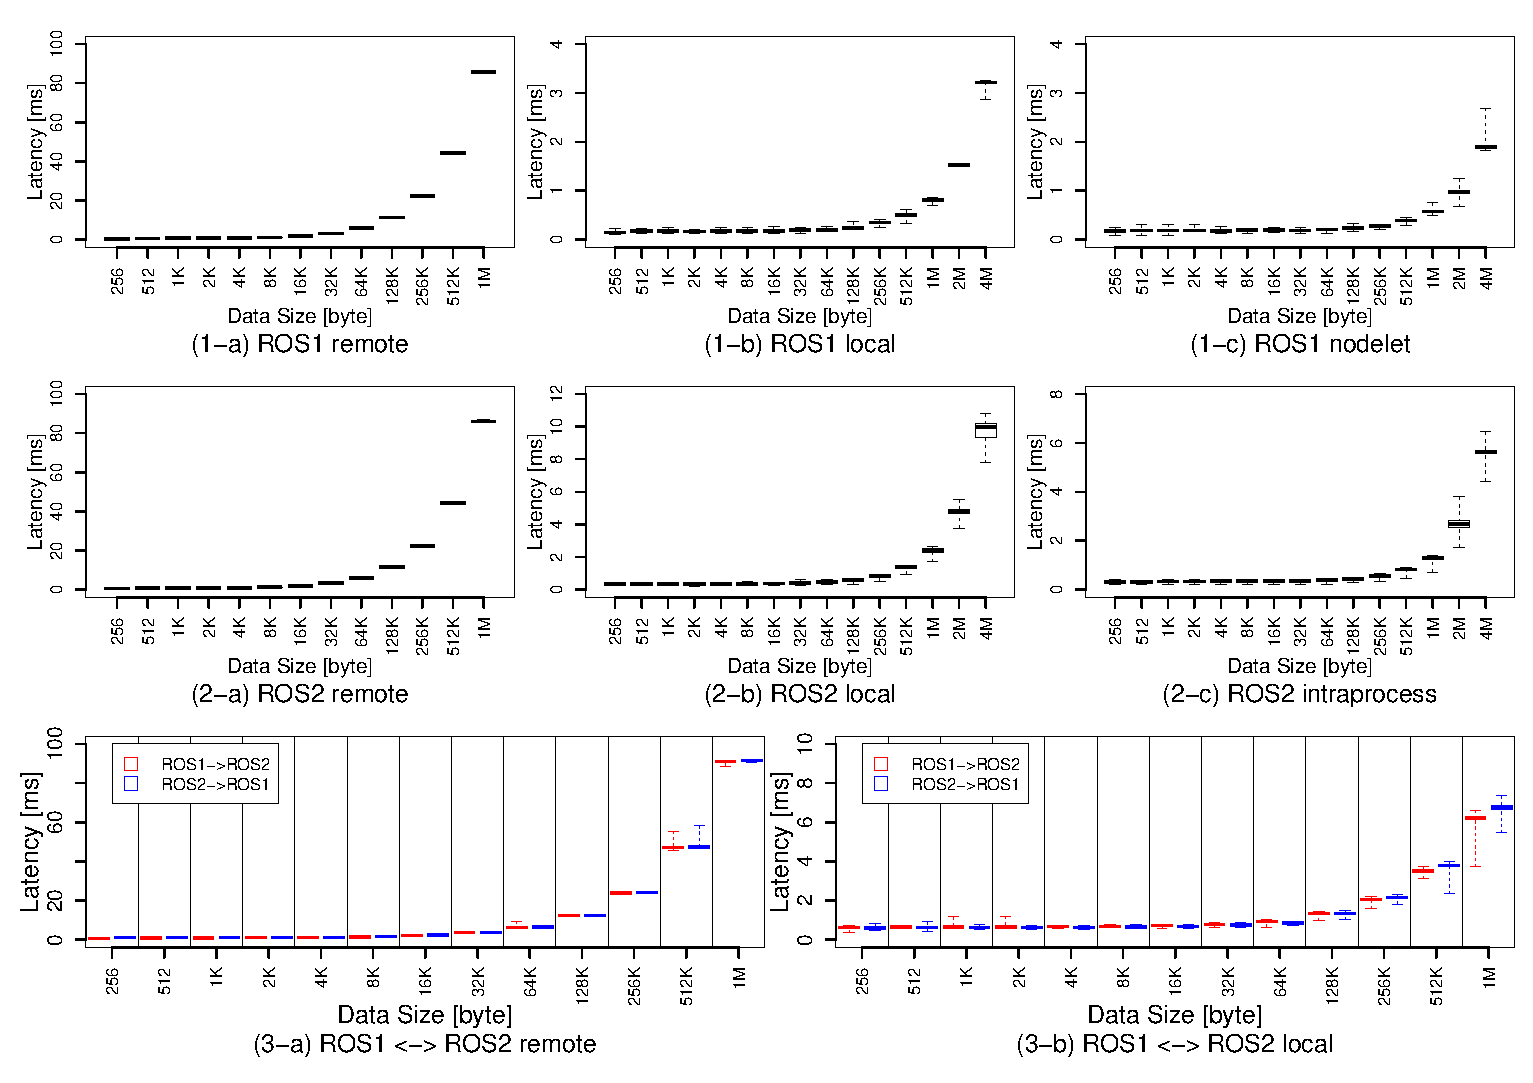
\includegraphics[width=1.0\linewidth]{../figure/overview_BoxPlot.eps}
%% \caption{\label{fig:overview_boxplot}
%% Overview of end-to-end latencies of ROS1 and/or ROS2.}
%% \end{figure*}


As shown in Figure \ref{fig:orgparagraph5}, various communication situations between \emph{nodes} in ROS1 and/or ROS2 are evaluated in the following experiments.
Whereas ROS1 is used in (1-a), (1-b), and (1-c), ROS2 is used in (2-a), (2-b), and (2-c). 
In (3-a) and (3-b), ROS1 and ROS2 \emph{nodes} coexist.
Note that the case of (2-c) does not require DDS due to \emph{intra-process communication}, i.e., shared memory transport.
Shared memory transport is used in the (1-c) \emph{nodelet} and (2-c) \emph{intra-process} cases.
In the experiments, \texttt{Machine1} is only used in (1-b), (1-c), (2-b), (2-c), and (3-b).
End-to-end latencies are measured on the same machine by sending \emph{messages} between \emph{nodes}.
\emph{Messages} pass over a local loopback in \texttt{local} cases, i.e.,  (1-b), (2-b), and (3-b).
Otherwise, for communication across the network, \texttt{Machine1} and \texttt{Machine2} are used in \texttt{remote} cases, i.e., (1-a), (2-a), and (3-a).
They are connected by a local IP network without any other network.

Communication between ROS1 and ROS2 \emph{nodes} requires a \texttt{ros\_bridge} \cite{ros2@roscon2015}, a \emph{bridge-node} that converts \emph{topics} for DDS. 
The \texttt{ros\_bridge} program has been released by the Open Source Robotics Foundation (OSRF) \cite{osrf}.
A \texttt{ros\_bridge} dynamically marshals several \emph{topics} for \emph{nodes} in ROS2. 
Thus, in (3-a) and (3-b), a \texttt{ros\_bridge} is launched on which ROS2 \emph{nodes} run.
Figure \ref{fig:orgparagraph6} shows the \emph{node}-graph for evaluation of communication from ROS1 to ROS2.
Note that a \texttt{best-effort policy} is the only one used when using a \texttt{ros\_bridge} because a \texttt{ros\_bridge} does not support the \texttt{RELIABLE} policy in the \emph{QoS Policy}. 

% In \texttt{remote} cases, to avoid time synchronization issues, the experiment adopts simple socket communication that routes through neither ROS1 nor ROS2.
% \texttt{Machine1} transmits data through ROS1 or ROS2, and receives short data through socket communication.
% In the adopted method, evaluation halts when \emph{messages} do not reach a \emph{subscriber-node} in the cases with, for example, the  \texttt{best-effort policy}, because a \emph{publisher-node} must wait until a \emph{subscriber-node} replies during each publish event.
% We estimate end-to-end latencies by subtracting preliminarily evaluated socket communication time.
% Using socket communication, the communication latencies between ROS1 and ROS2 can be evaluated respectively. 
% However, dividing round-trip latency in half cannot evaluate them and does not be used for this evaluation.
% Figure \ref{fig:orgparagraph6} shows the \emph{node}-graph for evaluation of communication from ROS1 to ROS2 with socket communication and a \texttt{ros\_bridge} in \texttt{remote} cases.

\vspace{-1mm}
\subsection{Capabilities of ROS1 and ROS2}
\label{sec:capacity}

Table \ref{tb:capabilities} shows whether end-to-end latencies can be measured for each data size with a comment about the causal factors of the experimental results.
Table \ref{tb:capabilities} summarizes ROS2's capabilities, and several interesting observations can be made.
In the ``Initial loss'' column, ROS1 fails to obtain initial \emph{messages} when a \emph{node} sends \emph{messages} for the first time even though ROS1 uses TCPROS with small data such as 256 B \textcolor{red}{and \emph{subscriber-node} is launched before a \emph{publisher-node} begins to send \emph{messages}.}
Although TCPROS is reliable for delivering intermediate \emph{messages}, it does not support reliable transport of initial \emph{messages}.
This influences ROS2 when using a \texttt{ros\_bridge}.
In contrast, ROS2 does not lose initial \emph{messages}, even when using large data such as 4 MB.
This proves the reliability of DDS.
\textcolor{red}{In \texttt{best-effort policy}, a \texttt{subscriber-node} must be launched before a \emph{publisher-node} begins to send \emph{messages} for ``Initial loss'' none.}
On the other hand, with ROS2 \texttt{reliable policy}, a \emph{subscriber-node} does not have to be launched before a \emph{publisher-node} starts sending \emph{messages}.
This is attributed to \texttt{TRANSIENT\_LOCAL} in DURABILITY of the \emph{QoS Policy}.
The \texttt{reliable policy} is tuned to provide resilience against late-joining \emph{subscriber-nodes}.
In ROS1, published \emph{messages} are lost and never recovered.
This \emph{QoS Policy} accelerates fault-tolerance.

Another interesting observation from Table \ref{tb:capabilities} is that ROS2 has many problems when transporting large data.
Many experiments fail in various situations with ROS2; however, we can observe differences in performance between Connext and OpenSplice.
These constraints on large data originate from the fact that the maximum payload of Connext and OpenSplice is 64 KB.
\textcolor{red}{This is the maximum packet size of IP protocol.
Is is hard to maintain divided packets with \emph{QoS Policy} by default API.}
Therefore, we consider that DDS is not designed to handle large data.
This is important for the analysis of ROS2 performance.
For example, FastRTPS does not support large data because it is designed as a lightweight implementation for embedded systems.
Even a string of 256 B exceeds the maximum length in FastRTPS.
Many DDS vendors do not support publishing large data with reliable connections and common APIs.
\textcolor{red}{To send and manage divided packets, such DDS vendors provide an alternate API such as an asynchronous publisher and flow controller, which has not been abstracted from ROS2.}
In our experiments, Connext with \texttt{reliable policy} yields errors when data are greater than 64 KB.
Some failures with the \texttt{best-effort policy} are due to frequent \emph{message} losses caused by non-reliable communication. 
When a \emph{publisher-node} fails to transfer data to a \emph{subscriber-node} frequently, we cannot collect sufficient samples and conduct evaluations.
Several evaluations fail in (3-b) and \texttt{remote} cases, as shown in Table \ref{tb:capabilities}.
Currently, the above results indicate that ROS2 is not suitable for handling large \emph{messages}.

\begin{figure*}[t]
  \tabcolsep = 0.5mm              % side-margin in column
  \begin{tabular}{ccc}
    \begin{minipage}[t]{0.32\textwidth}
      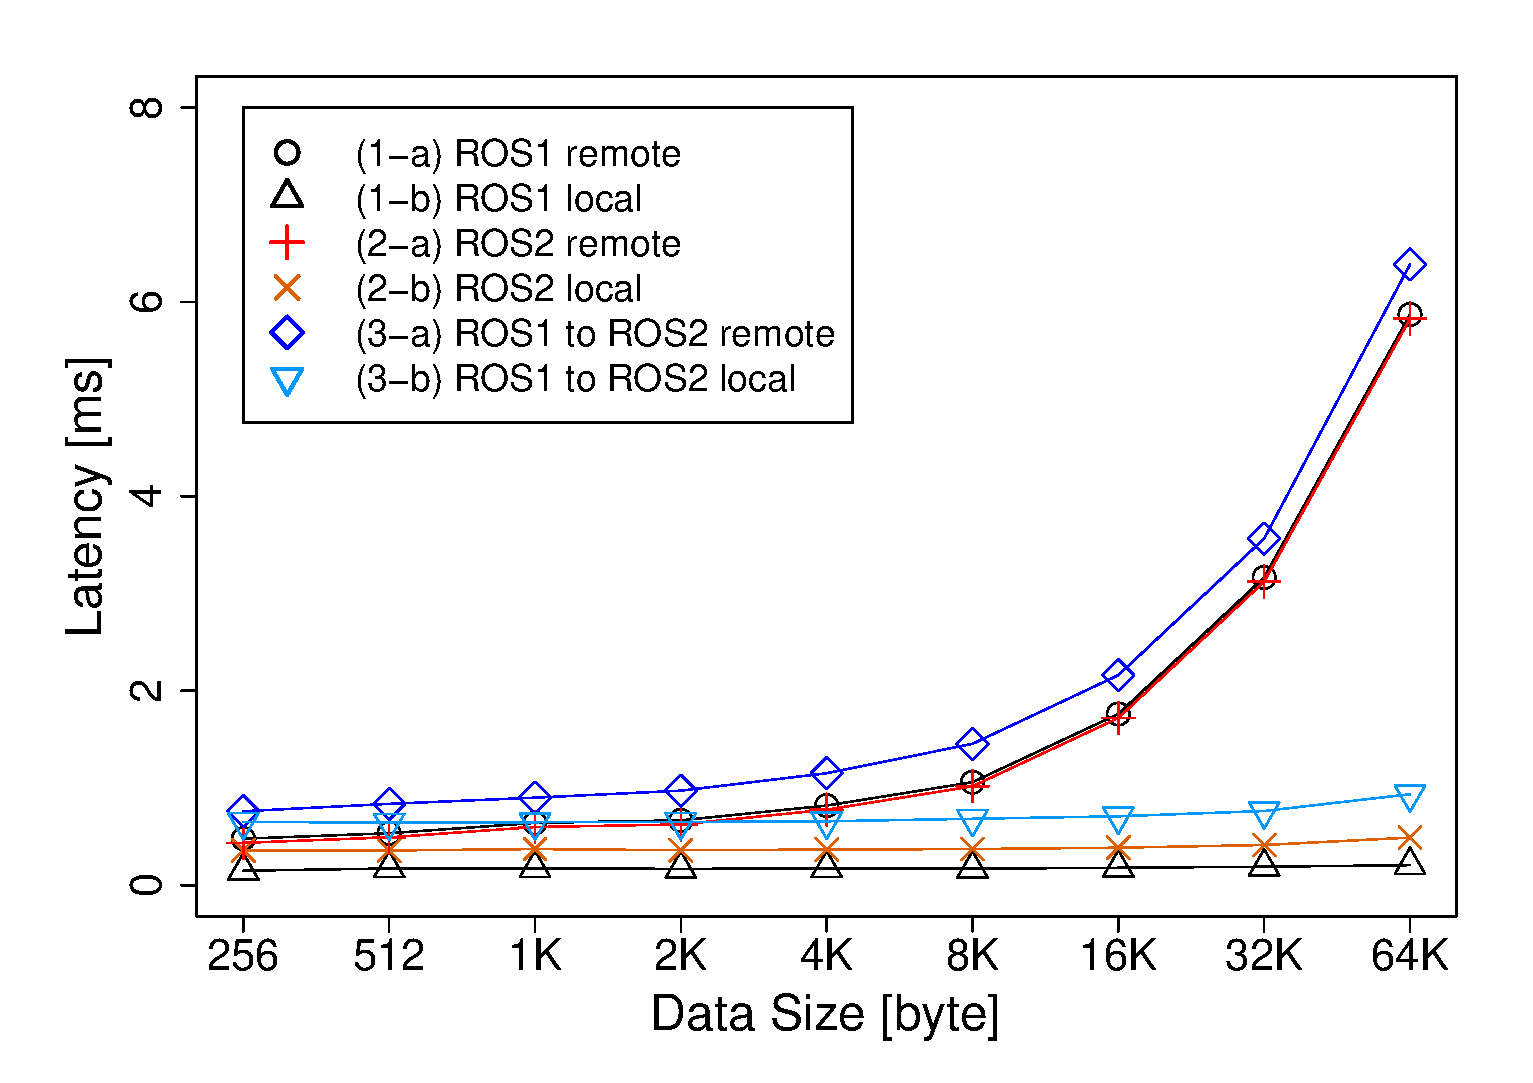
\includegraphics[width=1.0\linewidth]{../figure/comparison_remote_local_small-data_Plot.eps}
      \vspace{-7mm}
      \caption{Medians of end-to-end latencies with small data in \texttt{remote} and \texttt{local} cases.}
      \label{fig:remote_local_small_plot}
    \end{minipage}   
    &
    \setcounter{figure}{8}
    \begin{minipage}[t]{0.32\textwidth}
      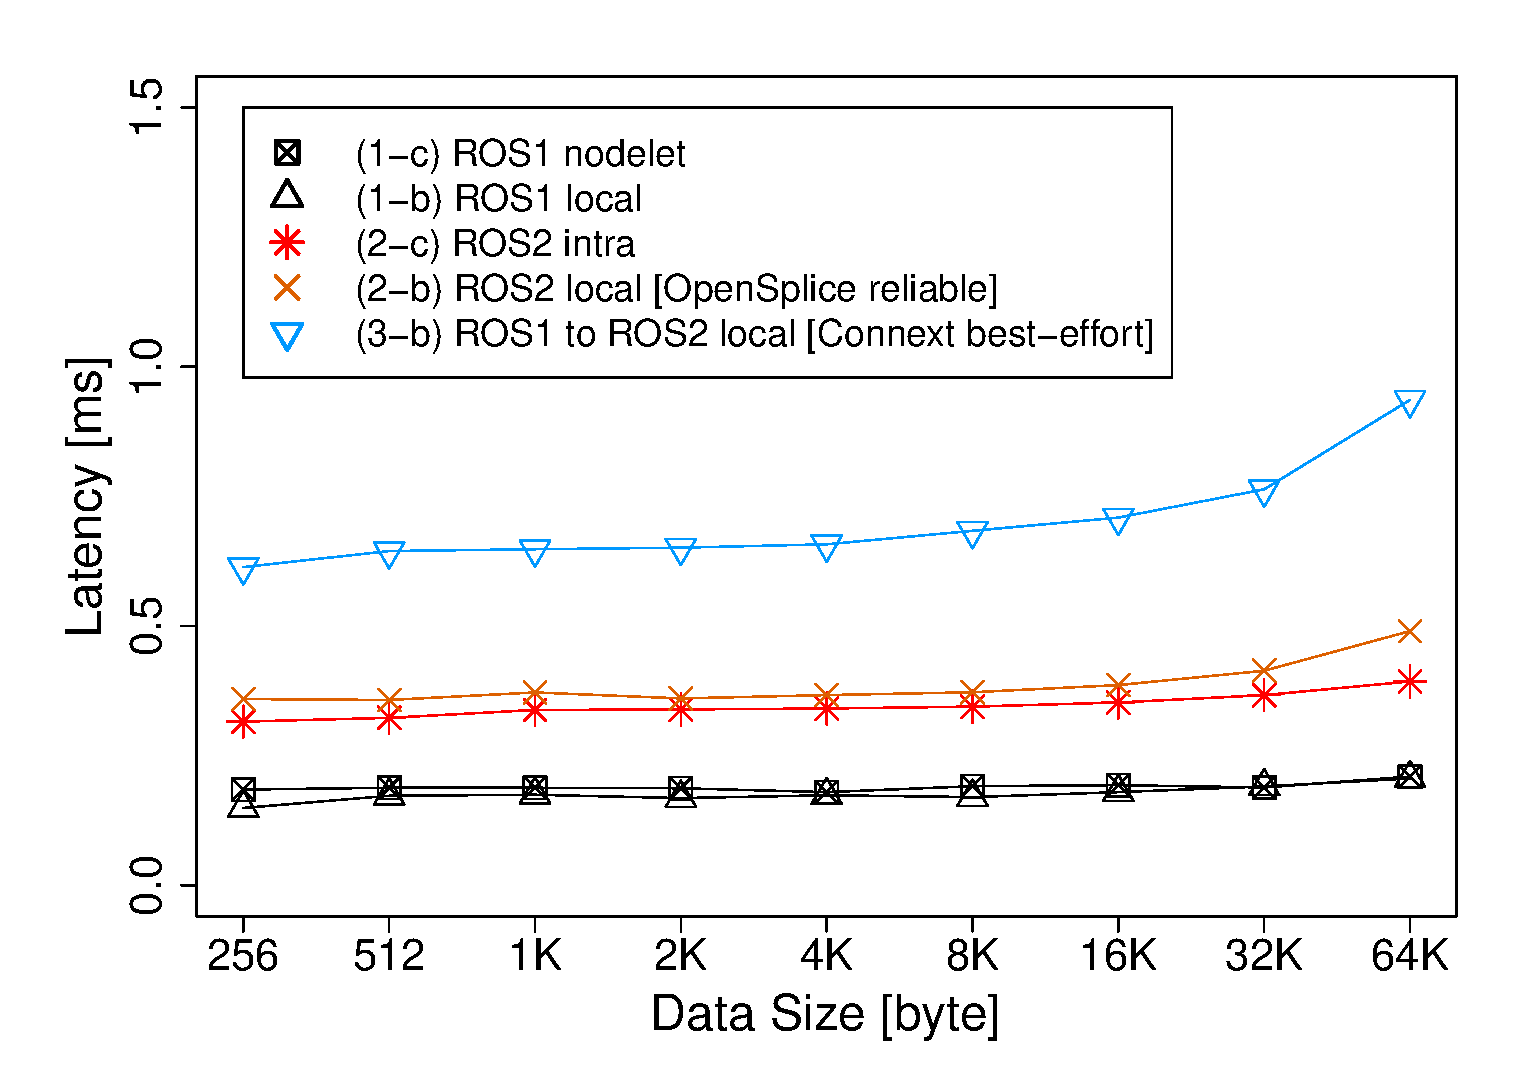
\includegraphics[width=1.0\linewidth]{../figure/comparison_intra_nodelet_local_small-data_Plot.eps}
      \vspace{-7mm}
      \caption{Medians of end-to-end latencies with small data in \texttt{local}, \emph{nodelet}, and \emph{intra-process} cases.}
      \label{fig:local_small_plot}
    \end{minipage}
    &
    \setcounter{figure}{10}
    \begin{minipage}[t]{0.32\textwidth}
      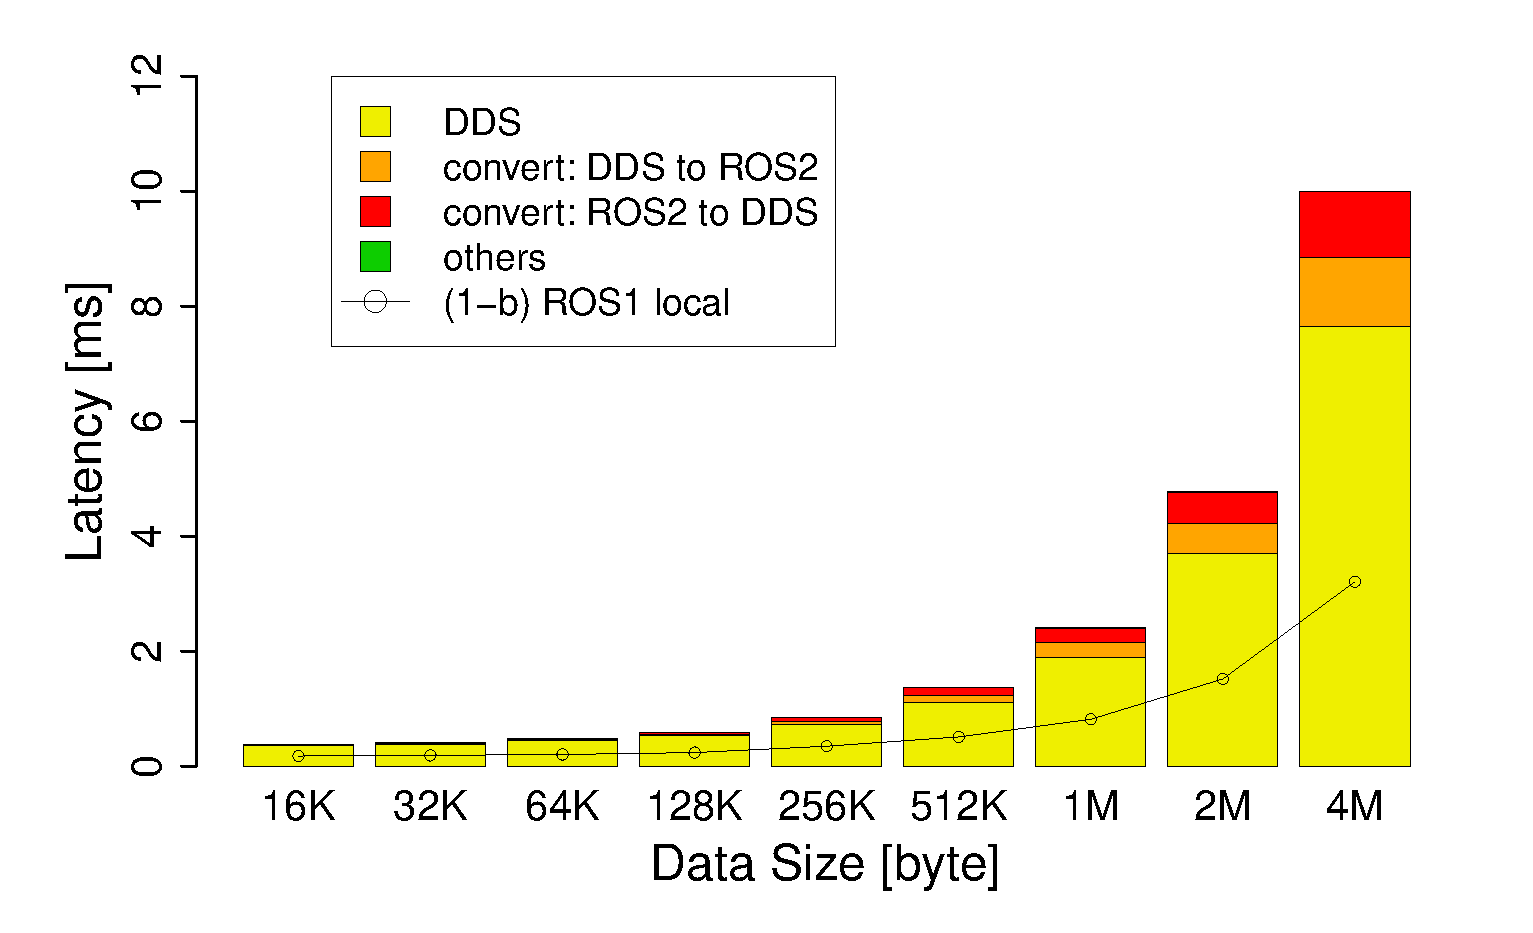
\includegraphics[width=1.0\linewidth]{../figure/breakdown_ros2_local_BarPlot.eps}
      \vspace{-7mm}
      \caption{(2-b) \texttt{reliable policy} breakdown of ROS2 latencies with the OpenSplice.}
      \label{fig:ros2_local_barplot}
    \end{minipage}
    \\  
    \setcounter{figure}{7}
    \begin{minipage}[t]{0.32\textwidth}
      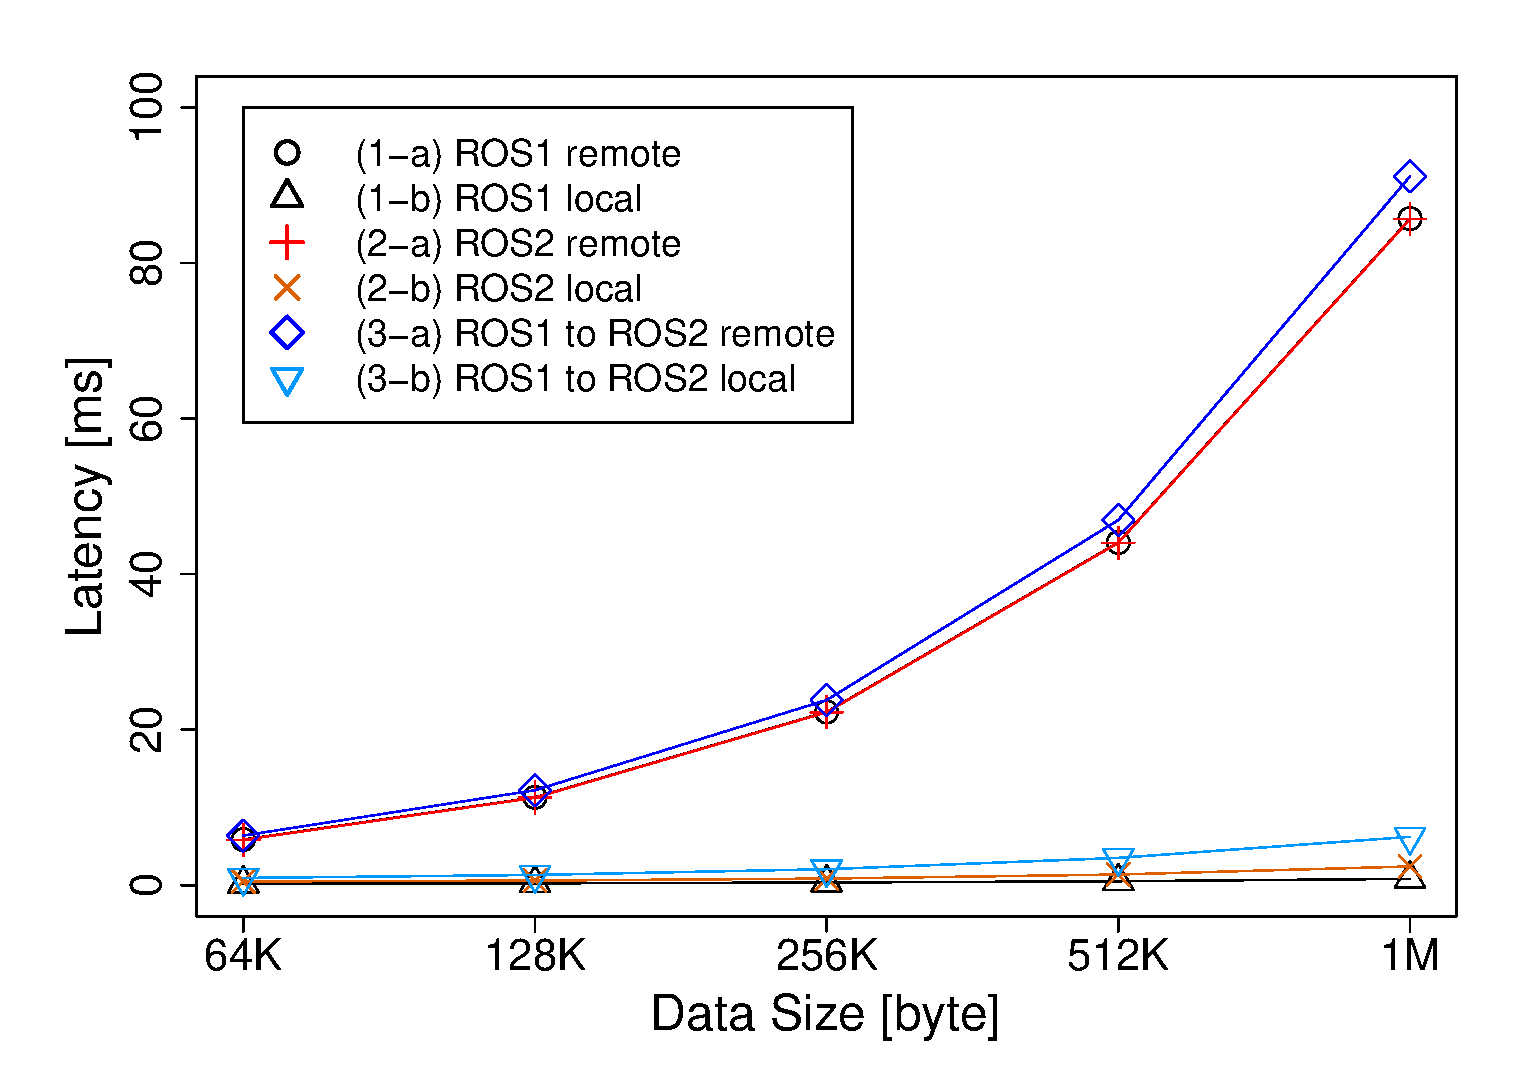
\includegraphics[width=1.0\linewidth]{../figure/comparison_remote_local_Plot.eps}
      \vspace{-7mm}
      \caption{Medians of end-to-end latencies with large data in \texttt{remote} and \texttt{local} cases.}
      \label{fig:remote_local_plot}
    \end{minipage}
    &
    \setcounter{figure}{9}
    \begin{minipage}[t]{0.32\textwidth}
      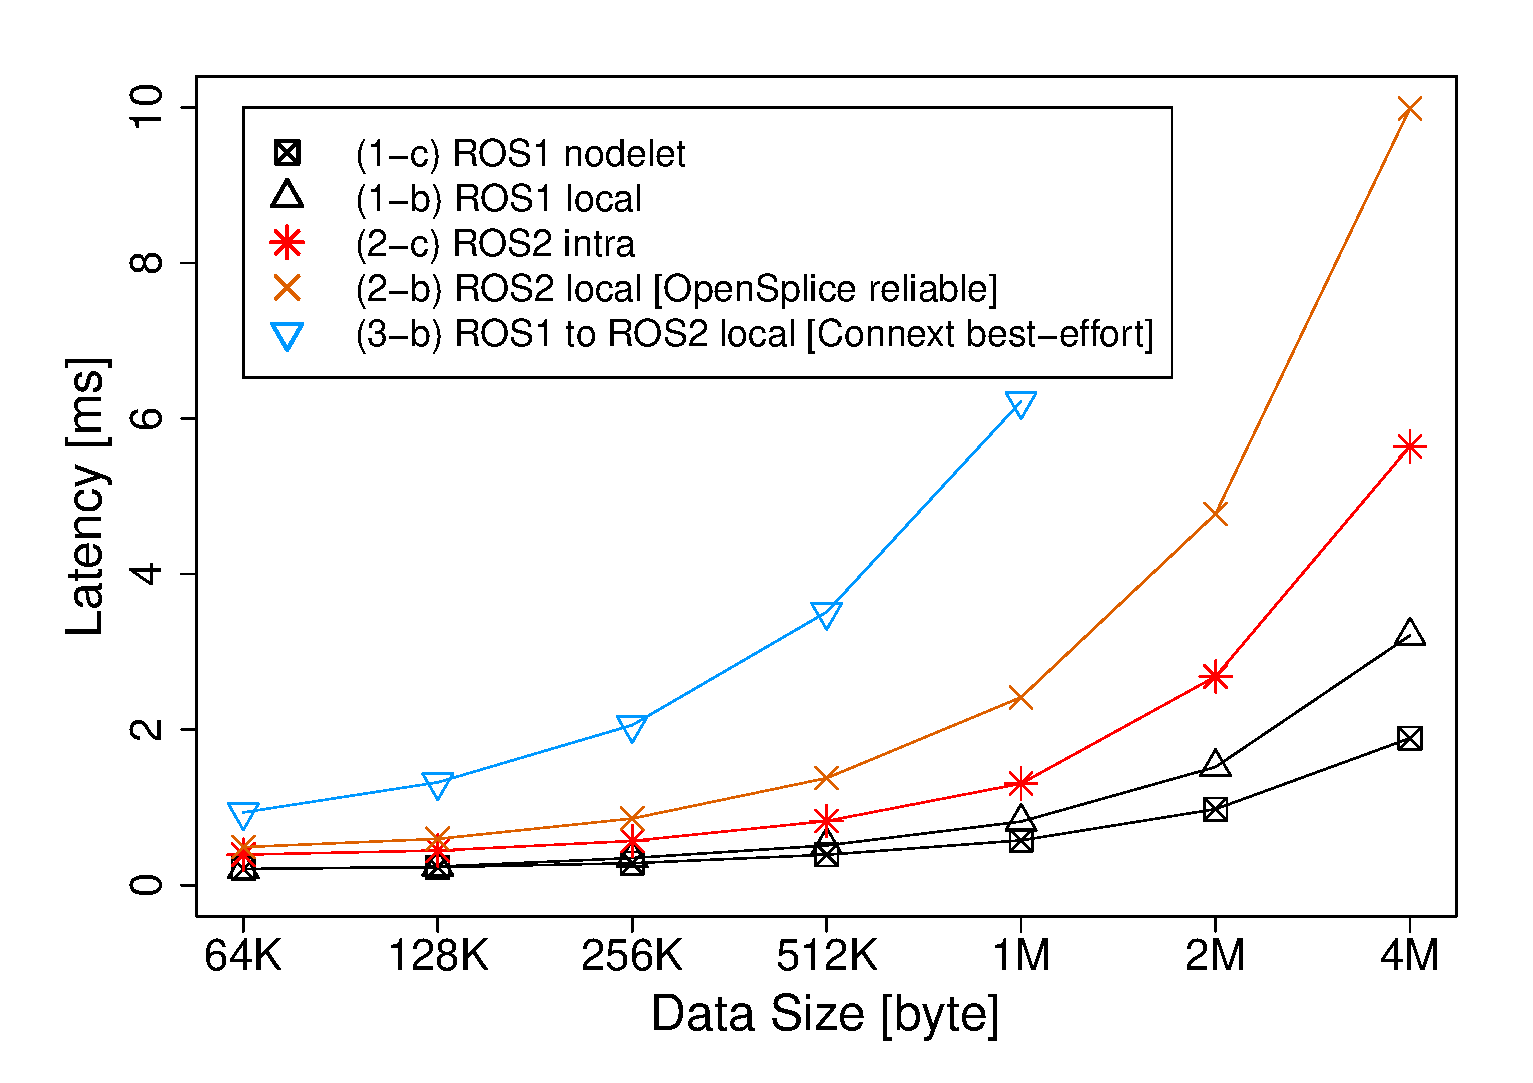
\includegraphics[width=1.0\linewidth]{../figure/comparison_intra_nodelet_local_Plot.eps}
      \vspace{-7mm}
      \caption{Medians of end-to-end latencies with large data in \texttt{local}, \emph{nodelet}, and \emph{intra-process} cases.}
      \label{fig:local_plot}
    \end{minipage}
    &
    \setcounter{figure}{11}
    \begin{minipage}[t]{0.32\textwidth}
      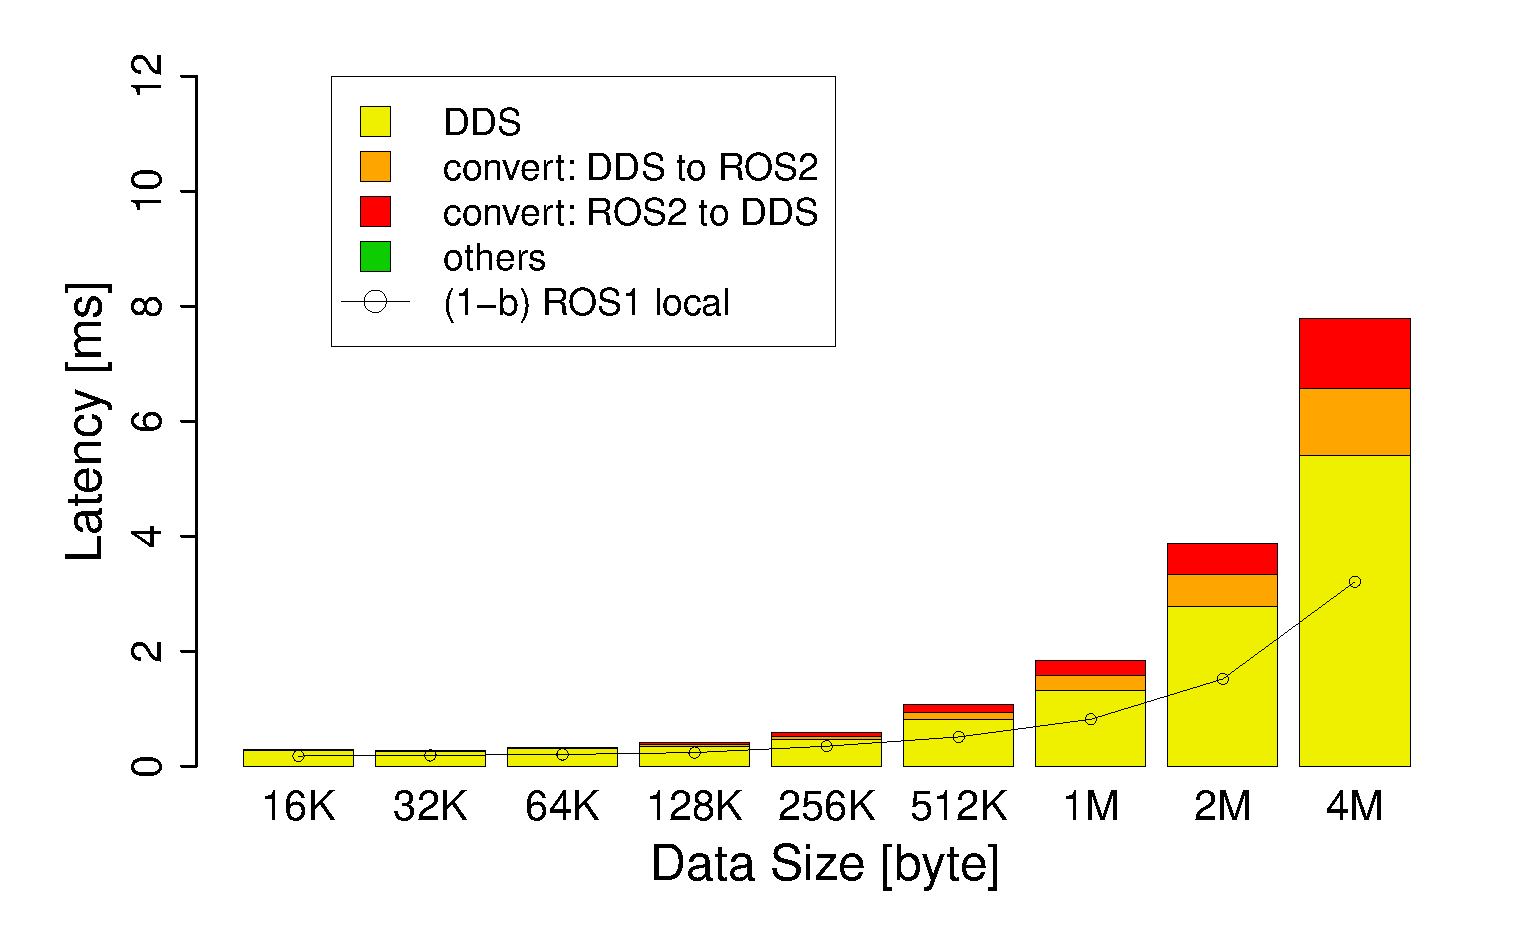
\includegraphics[width=1.0\linewidth]{../figure/breakdown_ros2_local_best-effort_BarPlot.eps}
      \vspace{-7mm}
      \caption{(2-b) \texttt{best-effort policy} breakdown of ROS2 latencies with the OpenSplice.}
      \label{fig:ros2_local_best-effort_barplot}
    \end{minipage}
    \vspace{-3mm}
  \end{tabular}
  \vspace{-2mm}
\end{figure*}

\vspace{-2mm}
\subsection{Latency Characteristics of ROS1 and ROS2}
\label{sec:latency}

As shown in Figures \ref{fig:remote_local_small_plot}, \ref{fig:remote_local_plot}, \ref{fig:local_small_plot}, \ref{fig:local_plot}, a tendency of end-to-end latencies characteristics is clarified in each situation shown in Figure \ref{fig:orgparagraph5}.
In (2-a) and (2-b), ROS2 uses OpenSplice with the \texttt{reliable policy}  because ROS1 uses TCPROS, i.e., reliable communication.
In (3-a) and (3-b), to evaluate latencies with large data (e.g., 512 KB and 1 MB), Connext with the \texttt{best-effort policy} is used.
First, we analyze ROS2 performance compared to ROS1.
We then evaluate ROS2 with different DDS implementations and configurations, such as the \emph{QoS Policy}.

% \noindent \textbf{Comparison between \texttt{remote} and \texttt{local} cases:} 
\vspace{-2mm}
\subsubsection{Comparison between \texttt{remote} and \texttt{local} cases}
\label{sec:remote_local}
ROS1 and ROS2 is much less than the difference between \texttt{remote} and \texttt{local} cases.
Figures \ref{fig:remote_local_small_plot} and \ref{fig:remote_local_plot} show the medians of the latencies for the \texttt{remote} and \texttt{local} cases.
Since the conversion influences from ROS1 to ROS2 and from ROS2 to ROS1 are similar, Figures \ref{fig:remote_local_small_plot} and \ref{fig:remote_local_plot} contain one-way data.
In Figure \ref{fig:remote_local_small_plot}, the behavior of all latencies is constant up to 4 KB.
In contrast, the latencies in the \texttt{remote} cases grow sharply from 16 KB, as shown in Figures \ref{fig:remote_local_small_plot} and \ref{fig:remote_local_plot}.
This is because ROS1 and ROS2 divide a message into 15 KB packets to transmit data through Ethernet.
This difference between the \texttt{remote} and \texttt{local} cases corresponds to the data transmission time between \texttt{Machine1} and \texttt{Machine2}, which was measured in a preliminary experiment. The preliminary experiment measured transmission time for each data size using ftp or http.
This correspondence indicates that the RTPS protocol and data about the \emph{QoS Policy} have little influence on data transmission time in the network.
In addition, all latencies are predictable by measuring the data transmission time.


% \noindent \textbf{Comparison among \texttt{local}, \emph{nodelet}, and \emph{intra-process} cases:}
\vspace{-3mm}
\subsubsection{Comparison among \texttt{local}, nodelet, and intra-process cases}
\label{sec:local}
The latencies characteristics differ in the cases of small and large data.
For discussion, we divide the graph into Figures \ref{fig:local_small_plot} and \ref{fig:local_plot}, which show the medians of the end-to-end latencies for local loopback and shared memory transport.
\textcolor{red}{This is because whether a \emph{message} is divided into several packets or not is an import issue to consider end-to-end latencies.}

For data size less than 64 KB, a constant overhead with ROS2 is observed, as shown in Figure \ref{fig:local_small_plot}, because DDS requires marshaling various configurations and decisions for the \emph{QoS Policy}.
We observe a trade-off between latencies and the \emph{QoS Policy} regardless of data size.
Although the \emph{QoS Policy} produces inevitable overhead, the latencies are predictable and small.
(3-b) has significant overhead due to the \texttt{ros\_bridge} transaction.
In the (3-b) case, a \texttt{ros\_bridge} incurs more overhead to communicate with ROS1 and ROS2.

With large data, ROS2 has significant overhead depending on the size of data, as shown in Figure \ref{fig:local_plot}.
The overhead of ROS2 in (2-b) is attributed to two factors, i.e., data conversion for DDS and processing DDS.
Note that ROS2 in (2-a) and (2-b) must convert \emph{messages} between ROS2 and DDS twice.
One conversion is from ROS2 to DDS, and the other conversion is from DDS to ROS2.
Between these conversions, ROS2 calls DDS APIs and passes \emph{messages} to DDS.
Figures \ref{fig:ros2_local_barplot} and \ref{fig:ros2_local_best-effort_barplot} show a breakdown of the end-to-end latencies in the (2-b) OpenSplice \texttt{reliable policy} and \texttt{best-effort policy}.
We observe that ROS2 requires only conversions and processing of DDS.
As shown in Figures \ref{fig:ros2_local_barplot} and \ref{fig:ros2_local_best-effort_barplot}, there are nearly no transactions for ``others''.
In addition, note that data size influences both conversions and the DDS processing.
Compared to ROS1, the DDS overhead is not constant, and the impact of DDS is notable with large data.
As a result, ROS2 has significant overhead with large data, while the impact of DDS depends on the \emph{QoS Policy}.

Furthermore, the influence of shared memory with large data is observed in Figure \ref{fig:local_plot}.
As data becomes large, notable differences can be observed.
However, the influence appears small in Figure \ref{fig:local_small_plot} because small data hides the impact of shared memory.

Another interesting observation is that the latencies in the (2-c) \emph{intra-process} are greater than the latencies in (1-b) despite using shared memory.
This result is not due to conversions for DDS and processing of DDS, because \emph{intra-process communication} does not route through DDS.
As ROS2 is in development, that gaps will be closed.
\emph{Intra-process communication} needs to be improved.

% \noindent \textbf{Comparison within ROS2:} 
\vspace{-2mm}
\subsubsection{Comparison within ROS2}
\label{sec:ros2}

\begin{figure*}[t]
  \tabcolsep = 1mm              % side-margin in column@
  \begin{tabular}{ccc}
    \begin{minipage}[t]{0.322\textwidth}
      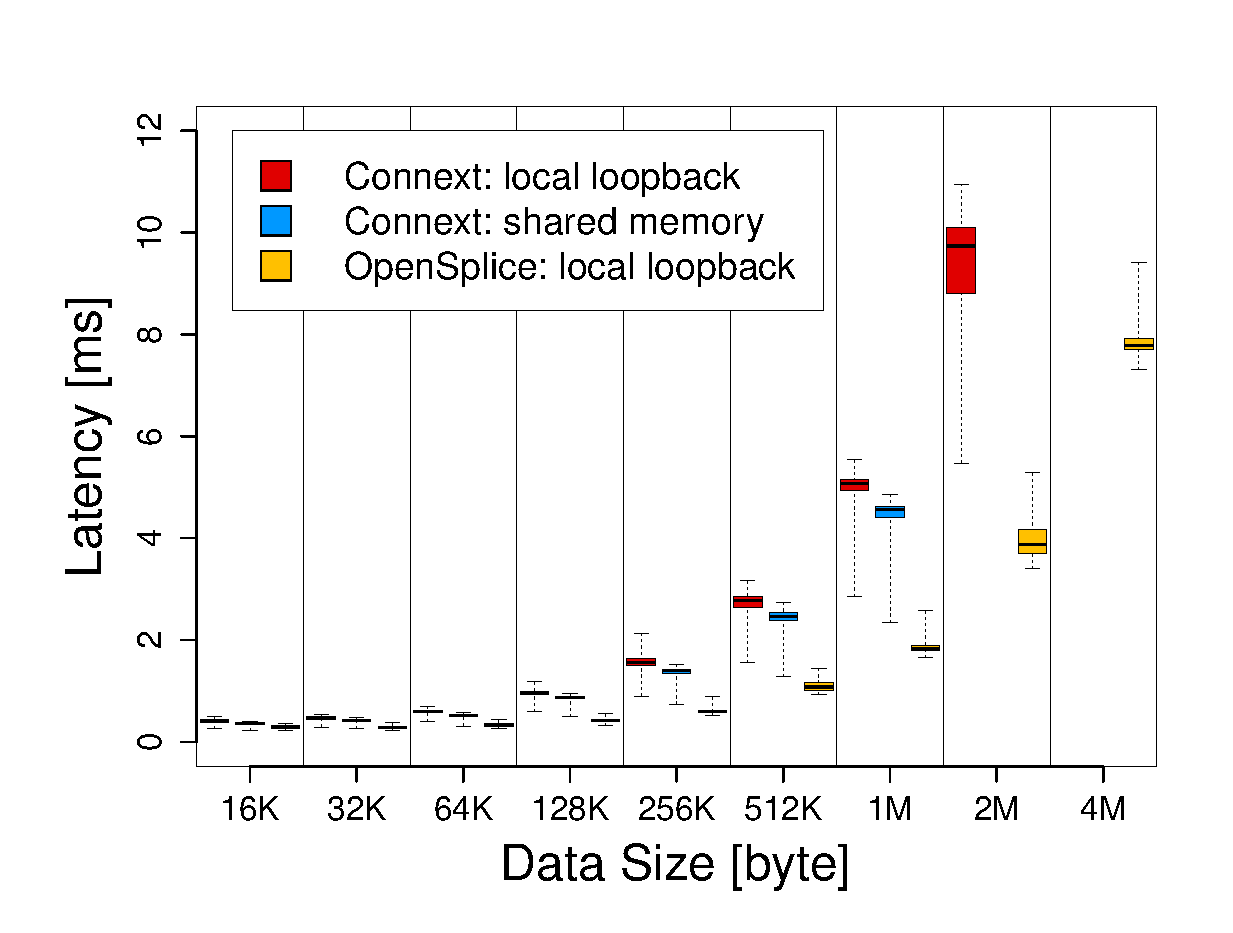
\includegraphics[width=1.0\linewidth]{../figure/comparison_DDS_BoxPlot.eps}
      \vspace{-7mm}
      \caption{(2-b) Different DDS in ROS2 with \texttt{best-effort policy}.}
      \label{fig:dds_boxplot}
    \end{minipage}
    &
    \begin{minipage}[t]{0.322\textwidth}
      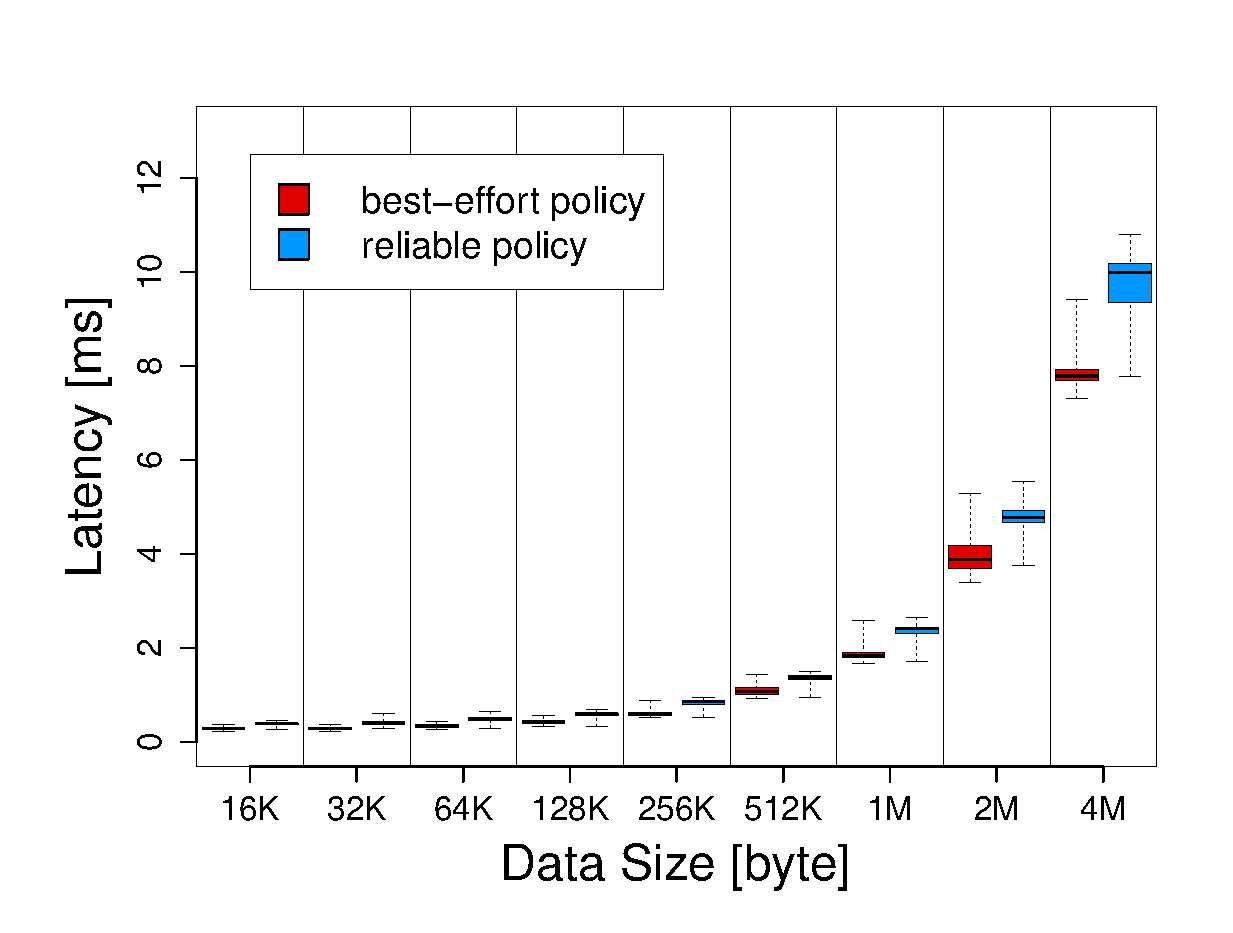
\includegraphics[width=1.0\linewidth]{../figure/comparison_qos_BoxPlot.eps}
      \vspace{-7mm}
      \caption{(2-b) Two \emph{QoS policies} in ROS2 with OpenSplice.}
      \label{fig:qos_boxplot}
    \end{minipage}
    &
    \textcolor{red}{
    \begin{minipage}[t]{0.322\textwidth}
      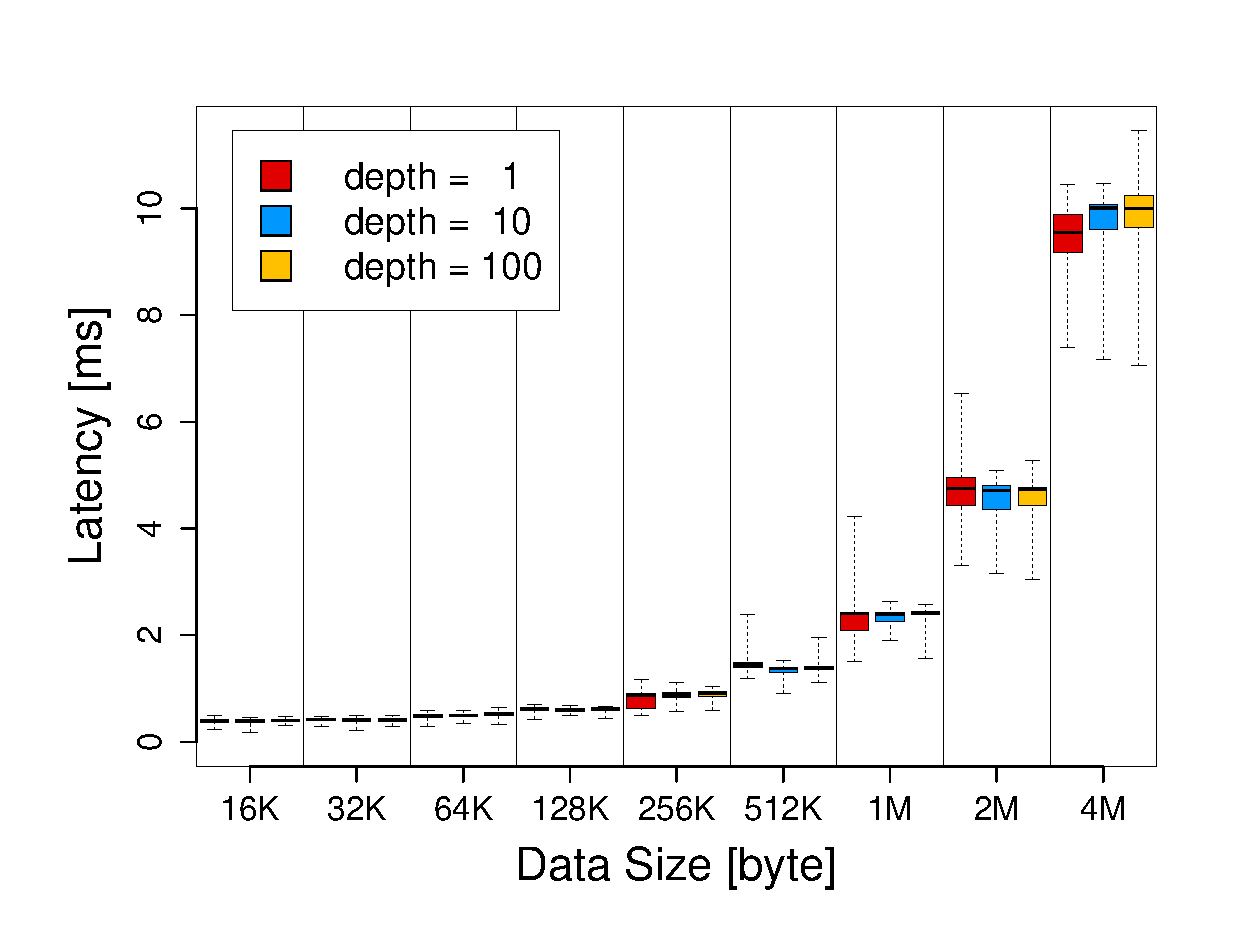
\includegraphics[width=1.0\linewidth]{../figure/BoxPlot_ospl_QoS_depth.eps}
      \vspace{-7mm}
      \caption{(2-b) Configured \texttt{*-depth policy} in ROS2 with OpenSplice.}
      \label{fig:depth_boxplot}
    \end{minipage}
    }
    \\
    \begin{minipage}[t]{0.322\textwidth}
      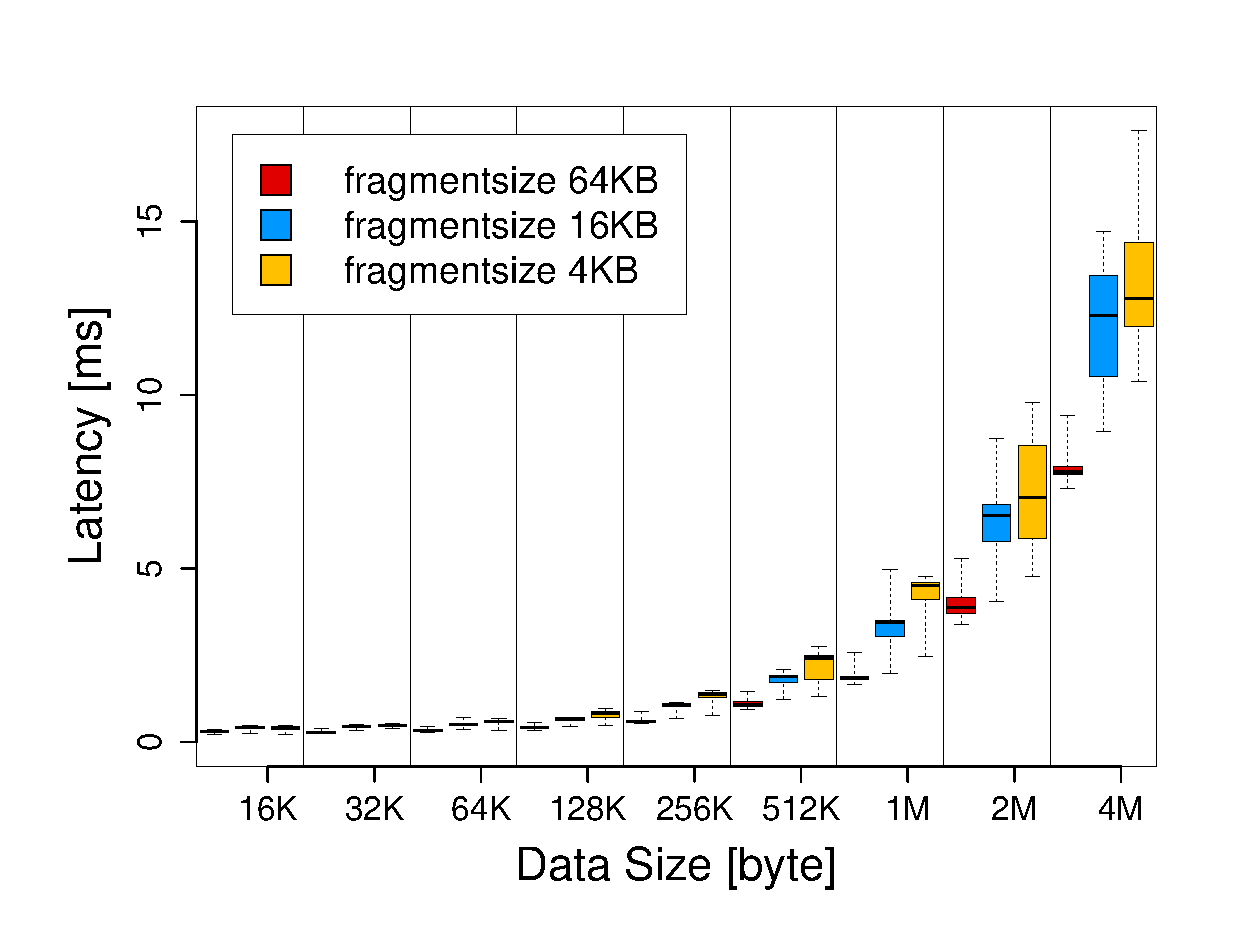
\includegraphics[width=1.0\linewidth]{../figure/comparison_ospl_frag_BoxPlot.eps}
      \vspace{-7mm}
      \caption{(2-b) Different fragment sizes in ROS2 with OpenSplice \texttt{best-effort policy}.}
      \label{fig:frag_boxplot}
    \end{minipage}
    &
    \textcolor{red}{
    \begin{minipage}[t]{0.322\textwidth}
      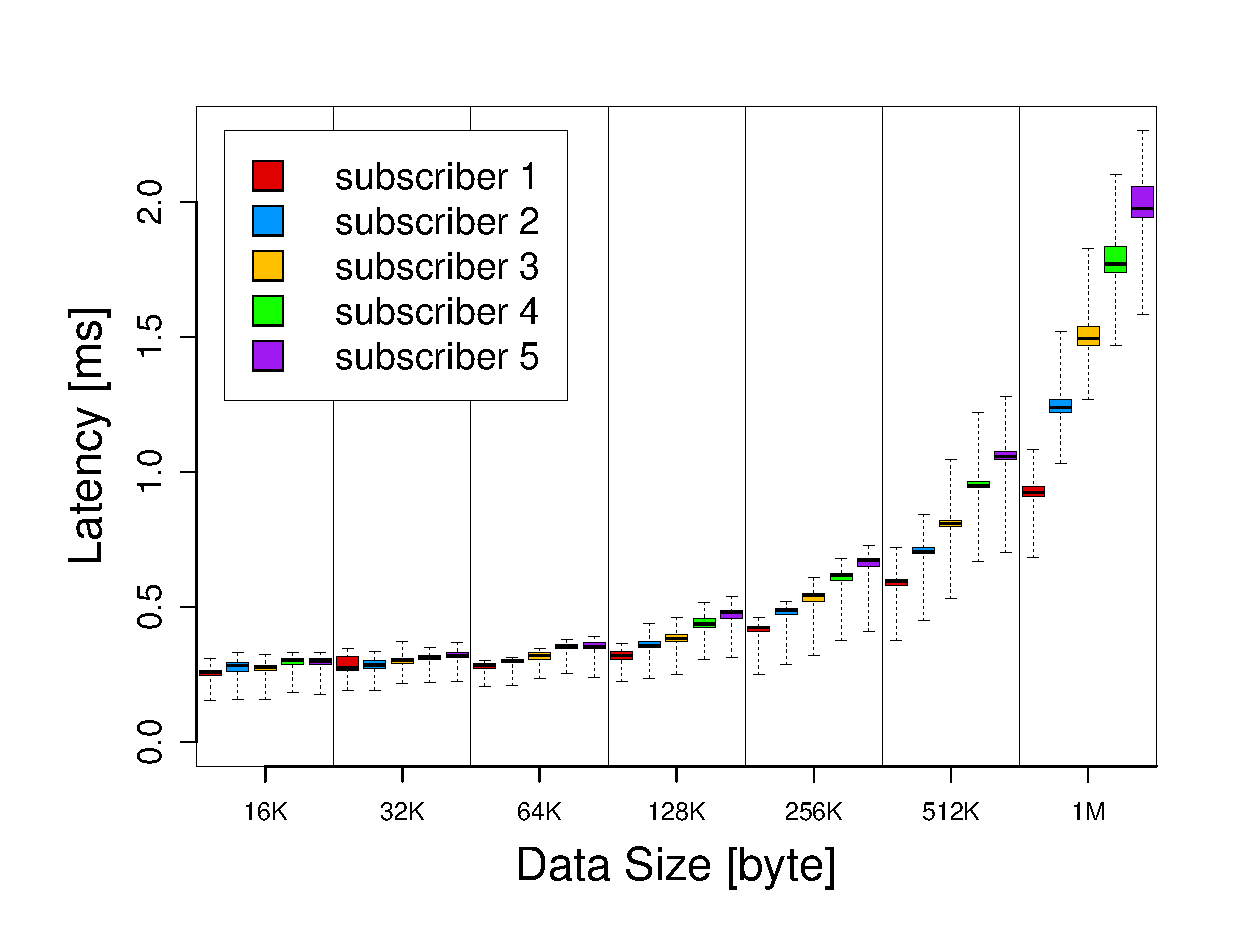
\includegraphics[width=1.0\linewidth]{../figure/BoxPlot_ros1_1M_multi-pub5.eps}
      \vspace{-7mm}
      \caption{(1-b) ROS1 multiple destinations publisher.}
      \label{fig:ros1_multi}
    \end{minipage}
    }
    &
    \textcolor{red}{
    \begin{minipage}[t]{0.322\textwidth}
      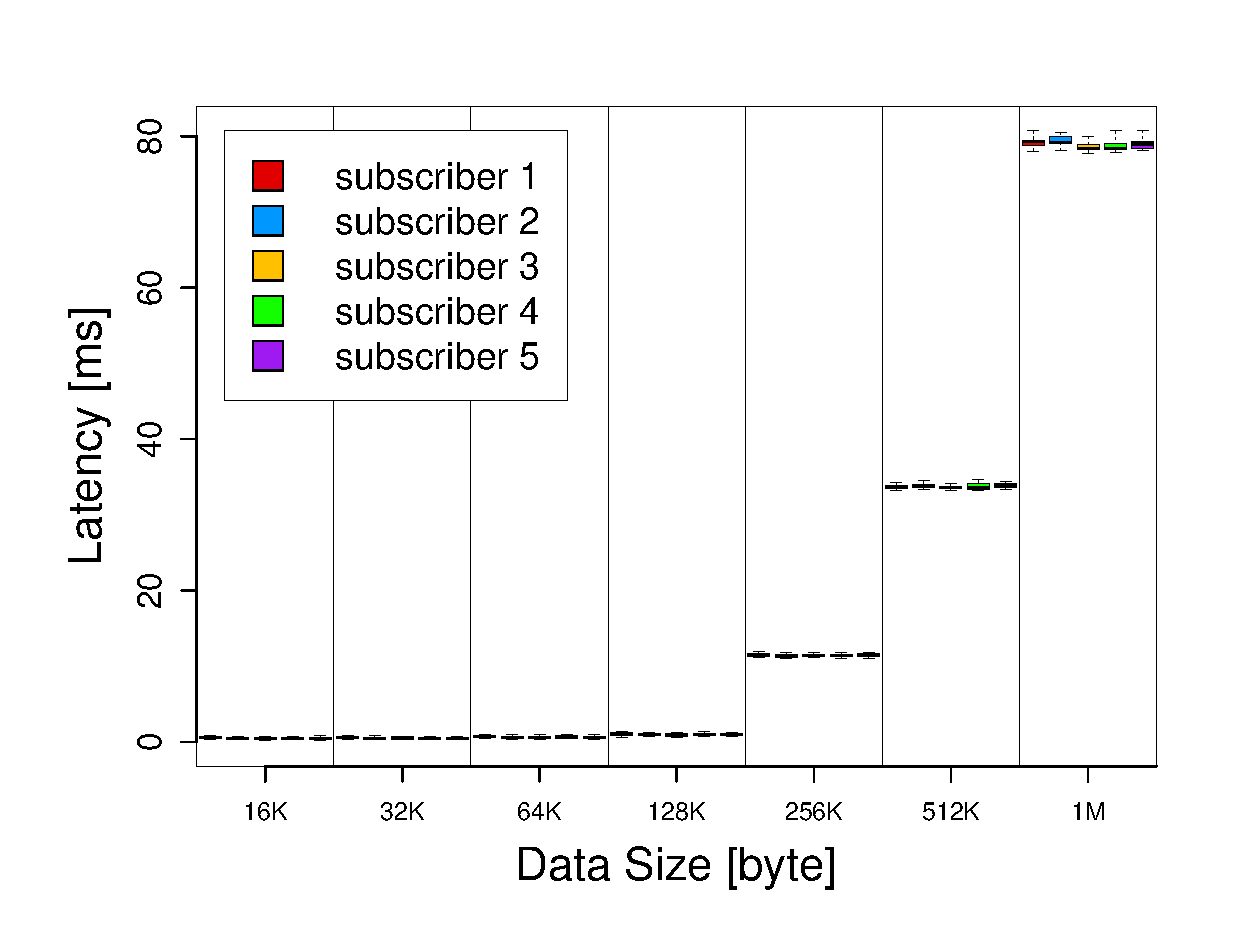
\includegraphics[width=1.0\linewidth]{../figure/BoxPlot_ospl_1M_multi-pub5.eps}
      \vspace{-7mm}
      \caption{(2-b) ROS2 multiple destinations with OpenSplice \texttt{reliable policy}.}
      \label{fig:ospl_multi}
    \end{minipage}
    }
    \vspace{-3mm}
  \end{tabular}
  \vspace{-3mm}
\end{figure*}

End-to-end latencies with data less than 16 KB exhibit similar performance in (2-b).
We discuss performance for data of 16 KB to 4 MB.

A comparison of different DDS implementations in (2-b) is shown in Figure \ref{fig:dds_boxplot}.
We evaluate OpenSplice and Connext with and without shared memory in (2-b) with the \texttt{best-effort policy}.
Despite shared memory, the performance is not significantly better than that of local loopback. 
This is caused by marshaling of various tools (e.g., logger and observer), even when using shared memory transport.
Moreover, OpenSplice is superior to Connext in terms of latency, as shown in Figure \ref{fig:dds_boxplot}, because we use Connext DDS Professional, which has much richer features than the OpenSplice DDS Community Edition.
\textcolor{red}{We assume that the performance of Vortex OpenSplice is similar to that of OpenSplice DDS Community Edition.
However, Vortex OpenSplice needs a commercial license and is not supported by ROS2.}

In addition, the influence of the \emph{QoS Policy} on end-to-end latencies is evaluated in (2-b) OpenSplice with the \texttt{reliable policy}, \texttt{best-effort policy}\textcolor{red}{, and \texttt{*-depth policy}.
\texttt{*-depth policy} is prepared for this evaluation and configured by depth as shown in Table \ref{tb:depth_qos}.
Figure \ref{fig:qos_boxplot} shows differences in latencies depending on the \texttt{reliable policy} and \texttt{best-effort policy}.}
The impact of the \emph{QoS Policy} is shown in Figures \ref{fig:ros2_local_barplot} and \ref{fig:ros2_local_best-effort_barplot}.
In this evaluation, the network is ideal, i.e., \emph{publisher-nodes} resend \emph{messages} very infrequently.
If the network is not ideal, latencies with the \texttt{reliable policy} increase.
The differences in RELIABILITY and DURABILITY in the \emph{QoS Policy} lead to overhead at the cost of reliable communication and resilience against late-joining \emph{Subscribers}.
\textcolor{red}{Figure \ref{fig:depth_boxplot} shows no differences depending on the depth of \texttt{*-depth policy}.
These \emph{QoS policies} are different in the number \emph{nodes} save \texttt{messages}.
Although this number influences resources, this does not affect latencies because archiving \emph{messages} is conducted in every publication.}

Finally, fragment overhead is measured using OpenSplice in (2-b) by changing the fragment size to the maximum UDP datagram size of 64 KB. 
A maximum payload for Connext and OpenSplice originates from this UDP datagram size, because dividing large data into several datagrams has significant impact on many implementations of the \emph{QoS Policy}.
As shown in Figure \ref{fig:frag_boxplot}, the end-to-end latencies are reduced, as fragment data size increases.
With a large fragment size, DDS does not need to split large data into many datagrams, which means fewer system calls and less overhead.
In terms of end-to-end latencies, we should preset the fragment size to 64 KB when using large data.


\vspace{-2mm}
\subsubsection{\textcolor{red}{Multiple Destinations Publisher in \texttt{local} cases}}
\label{sec:multiple}
\textcolor{red}{
In this section, we prepare five \emph{subscriber-nodes} and measure latencies of each \emph{node}.
Much of information shared in real applications is destinated to multiple destinations.
Hence, this evaluation is practical for user.
Figure \ref{fig:ros1_multi} shows latencies of ROS1.
We can observe significant differences between \emph{subscriber-nodes}.
This means ROS1 schedules \emph{message} publication in order and is not suitable for real-time systems.
For example, in 1 MB, subscriber 5 is about twice as mach as subscriber 1.
In contrast, ROS2 has small differences as shown in Figure \ref{fig:ospl_multi}.
All subscribers' behavior is fair in ROS2.
However, ROS2 latencies significantly depends on the number of packets.
This is same characteristic we learned from Figure \ref{fig:remote_local_plot}.
Figure \ref{fig:ospl_multi_128K} indicates fair latencies and dependency of packets.
Although we cannot say that latencies variance of ROS1 is larger than one of ROS2 due to the difference of the scale, Figures \ref{fig:ros1_multi}, \ref{fig:ospl_multi}, and \ref{fig:ospl_multi_128K} prove ROS2 \emph{message} publication is more fair to multiple subscribes than ROS1 one.
}

\vspace{-2mm}
\subsection{\textcolor{red}{Throughput of ROS1 and ROS2}}
\label{sec:throughput}
\textcolor{red}{
We also measure each throughput of ROS1 and ROS2 in the \texttt{remote} case.
In our one-way \emph{message} transport experiment, maximum bandwidth of the network is 12.5 MB/sec because we use 100 Mbps Ethernet (100BASE-TX) and Full-Duplex as shown in Table \ref{tb:environment}.
Nodes repeatedly transport each \emph{message} with 10Hz.
}

\textcolor{red}{
In small data from 256 B to 2 KB, we can observe a constant gap among ROS1, ROS2 with OpenSplice, and ROS2 with Connext from Figure \ref{fig:throughput_small}.
These additional data correspond with RTPS packets for \emph{QoS Policy} and heartbeat.
Hence, these gap does not depend on data size.
Moreover, Connext throughput is lower than OpenSplice one.
This becomes a big impact when users handle many kinds of small data with high Hz and/or network bandwidth is limited.
}

\textcolor{red}{
In large data from 2 KB to 4MB, curves of Figure \ref{fig:throughput_large} demonstrate sustainable theoretical throughput.
ROS2 and ROS2 is able to utilize all of available bandwidth and similarly behave in this situation.
Throughput is limited by the network and not by DDS.
}

\renewcommand{\arraystretch}{1.0}
\begin{table}[t]
  \caption{\label{tb:depth_qos}\textcolor{red}{Depth Configurable QoS Policies}}
  \centering
  \tabcolsep = 1.5mm              % side-margin in column
  \textcolor{red}{
  \begin{tabular}{c|c}
    \hline
    & \textbf{\texttt{*-depth policy} }\\
    \hline
    \hline
    DEADLINE & \texttt{100 ms}\\
    HISTORY & \texttt{LAST}\\
    depth & 1, 10, or 100\\
    RELIABILITY & \texttt{RELIABLE}\\
    DURABILITY & \texttt{TRANSIENT\_LOCAL}\\
    \hline
  \end{tabular}
  }
  \vspace{-5mm}
\end{table}

\begin{figure*}[t]
  \textcolor{red}{
  \begin{tabular}{ccc}
    \begin{minipage}[t]{0.32\textwidth}
      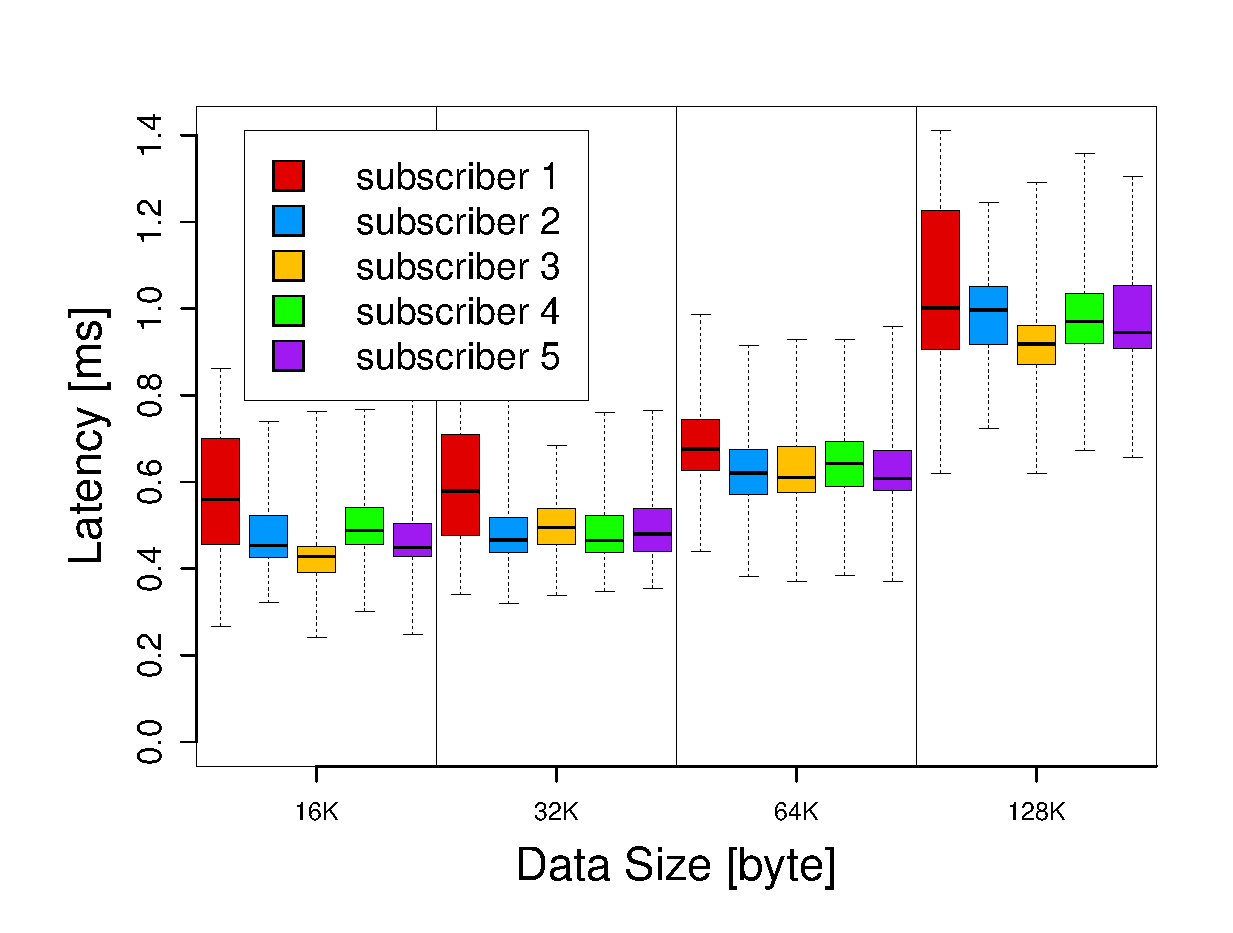
\includegraphics[width=1.0\linewidth]{../figure/BoxPlot_ospl_128K_multi-pub5.eps}
      \vspace{-7mm}
      \caption{(2-b) ROS2 multiple destinations with OpenSplice \texttt{reliable policy}.}
      \label{fig:ospl_multi_128K}
    \end{minipage}
    &
    \begin{minipage}[t]{0.32\textwidth}
      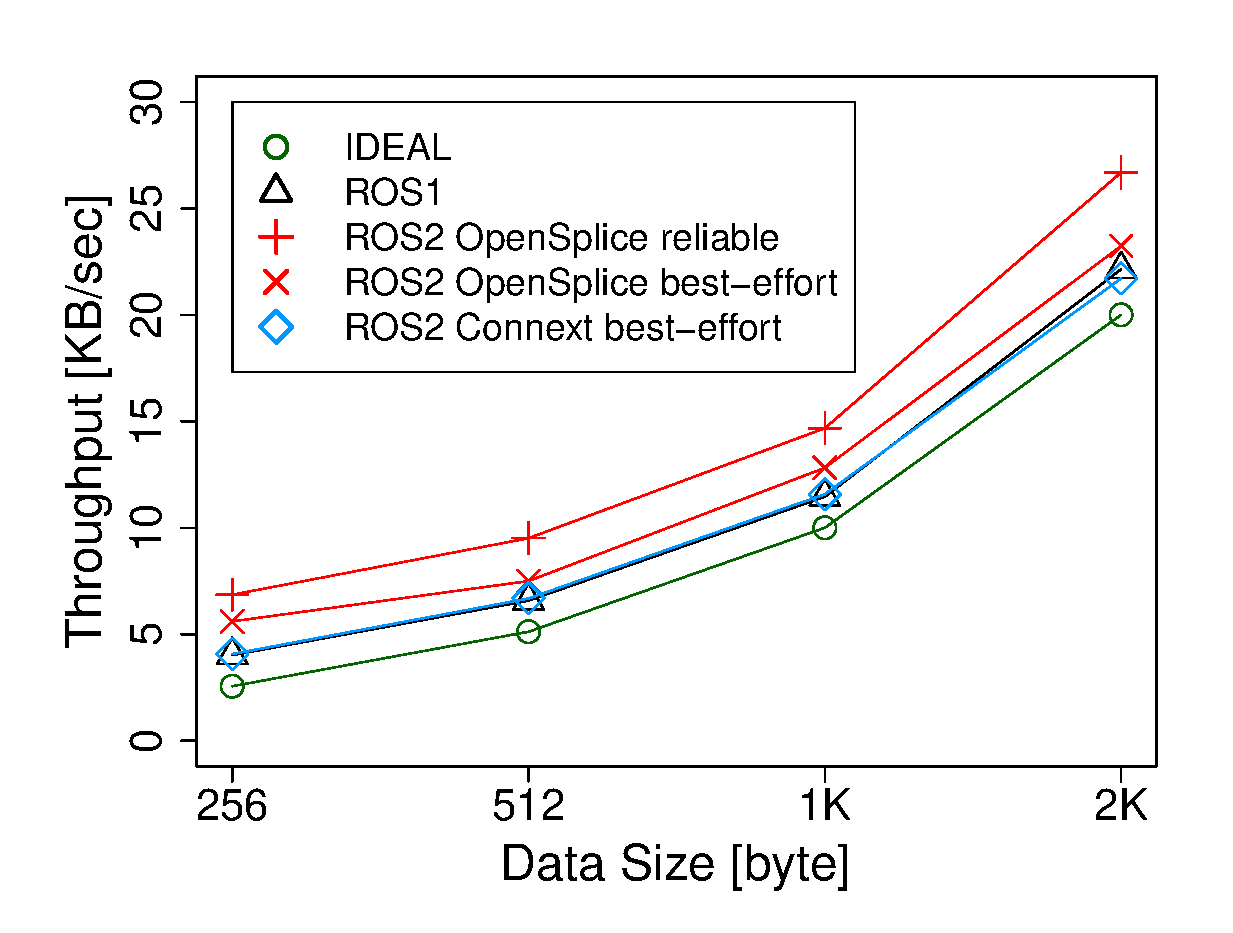
\includegraphics[width=1.0\linewidth]{../figure/throughput_remote_small-data.eps}
      \vspace{-7mm}
      \caption{(1-a) and (2-b) \texttt{remote} cases throughput with small data.}
      \label{fig:throughput_small}
    \end{minipage}
    &
    \begin{minipage}[t]{0.32\textwidth}
      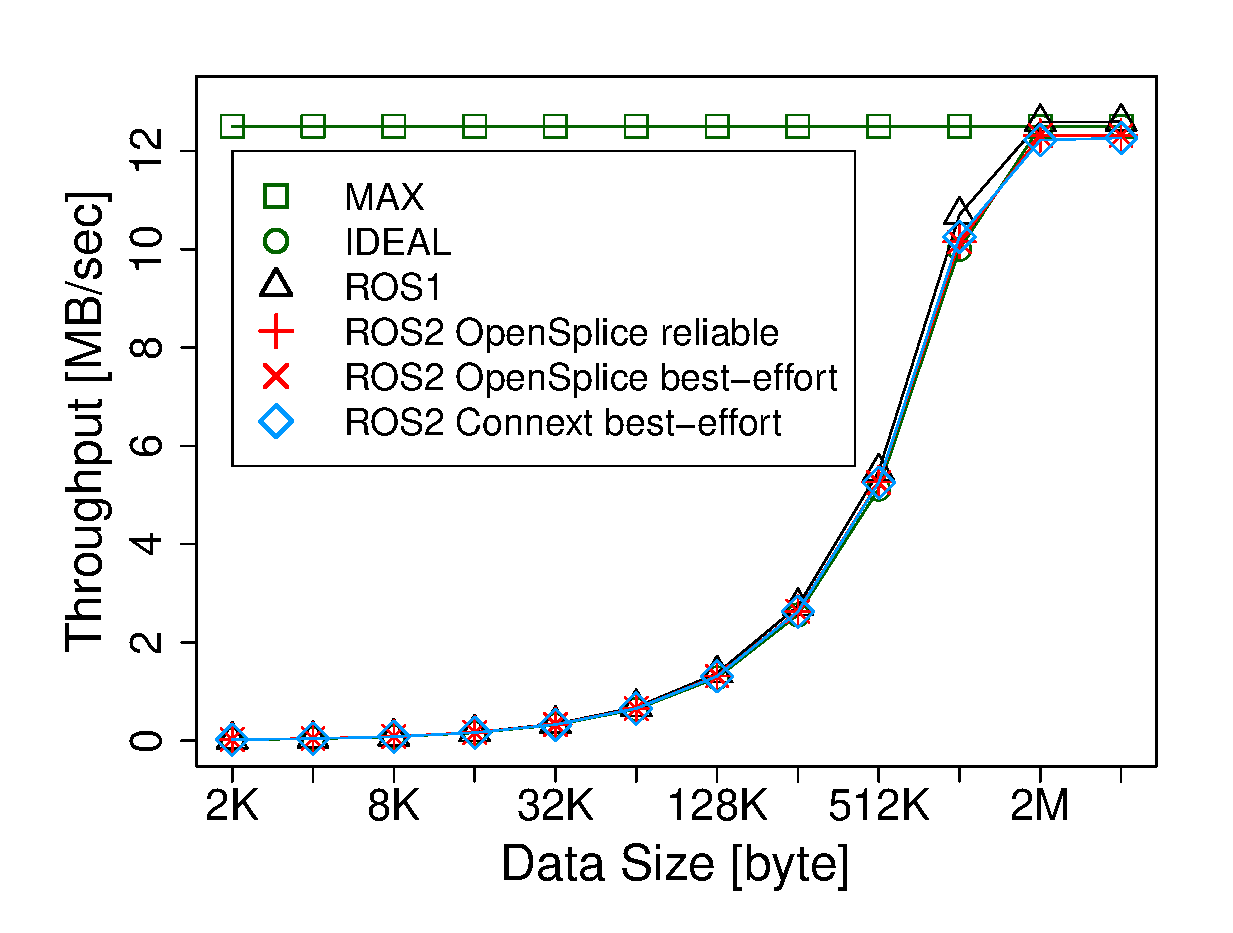
\includegraphics[width=1.0\linewidth]{../figure/throughput_remote_large-data.eps}
      \vspace{-7mm}
      \caption{(1-a) and (2-b) \texttt{remote} cases throughput with large data.}
      \label{fig:throughput_large}
    \end{minipage}
  \end{tabular}
  }
  \vspace{-8mm}
\end{figure*}


\vspace{-1mm}
\subsection{\textcolor{red}{Thread of ROS1 and ROS2}}
\label{sec:throughput}
\textcolor{red}{
In this section, we measure the number of threads on each \emph{node}.
Table \ref{tb:thread} shows the result of measurements.
Note that the number described in Table \ref{tb:thread} depends on DDS configuration including \emph{QoS Policy}.
The number does not be fixed by vendors.
}

\textcolor{red}{
First of all, we can observe that ROS2 \emph{node} with OpenSplice has a lot of threads.
This may cause parallelized processing and the fact that OpenSplice is much faster than Connext as shown in Figure \ref{fig:dds_boxplot}.
}

\textcolor{red}{
Another interesting point is FastRTPS threads.
ROS2 \emph{node} with FastRTPS realizes discovery and serialization, and pub/sub data transport with the same number of ROS1 \emph{node} threads.
This result proves improvement of fault tolerance without additional resources because FastRTPS does not need \emph{master-node}.
}
%% \renewcommand{\arraystretch}{1.1}
\begin{table}[t]
  \caption{\label{tb:thread}\textcolor{red}{The Number of Thread on ROS1 or ROS2}}
  \centering
  \tabcolsep = 1.5mm              % side-margin in column
  \textcolor{red}{
  \begin{tabular}{c|cccc}
    \hline
    & ROS1 & Connext & OpenSplice & FastRTPS \\
    \hline
    \hline
    node & 5 & 8 & 49 & 5 \\
    master-node & 3 & - & - & - \\
    \hline
  \end{tabular}
  }
  \vspace{-5mm}
\end{table}

\vspace{-1mm}
\subsection{\textcolor{red}{Memory consumption of ROS1 and ROS2}}
\label{sec:throughput}
\textcolor{red}{
We also measure memory size of shared library object (\texttt{.so}) in ROS1 and ROS2.
Shared libraries are libraries that are dynamically loaded by \emph{nodes} when they start.
They are not linked to executable files but they will be vital guidelines for estimation of memory size.
We arrange the result in Table \ref{tb:memory}.
In this table, we add up library data size for pub/sub transport.
In ROS2, shared libraries are classified into the DDS library and the ROS2 abstraction library.
While DDS libraries are provided by each vendor, ROS2 libraries abstract DDS APIs and convert \emph{messages} for DDS.
In Table \ref{tb:memory}, DDS and ROS2 libraries vary depending on vendors.
These library data size tends to increase because its QoS capability and abstraction.
For small embedded systems, we need a minimal DDS implementation and light abstraction layer.
}
\begin{table}[t]
  \caption{\textcolor{red}{Memory of .so Files for ROS1 and ROS}}
  \centering
  \renewcommand{\arraystretch}{1.15}
  \label{tb:memory}
  \small
  \tabcolsep = 1.0mm              % side-margin in column
  \textcolor{red}{
  \begin{tabular}{c|c||r|r||r}
    \hline
    \multicolumn{2}{c||}{} & DDS [KB] & Abstraction [KB] & Total [MB] \\ \hline \hline
    \multicolumn{2}{c||}{ROS1}  & \multicolumn{2}{c||}{ 2,206 } & 2.26 \\ \hline
    \multirow{3}{*}{ROS2} & Connext & 11,535 & 9,645 & 21.18 \\ 
    & OpenSplice & 3,837 & 14,117 & 17.95 \\ 
    & FastRTPS & 1,324 & 3,953 & 5.28\\ \hline
  \end{tabular}
  }
  \vspace{-5mm}
\end{table}


\vspace{-1mm}
\subsection{\textcolor{red}{Lessons Learned}}
\label{sec:lessons}
\textcolor{red}{
So far, we have clarified characteristic of DDS implementations through ROS2 from several standpoints: ROS2 capability, latencies, throughput, the number of threads and memory consumption.
We can get insight and guidelines for DDS through ROS2 from experimental results.
They will be meaningful for DDS and ROS users.
}

\textcolor{red}{
DDS supports \emph{QoS Policy} but there is trade-off of end-to-end latencies and throughput.
In the \texttt{local} case, overhead latencies of ROS2 is not trivial.
From Section \ref{sec:latency}, the latencies is caused by two data conversions for DDS and DDS transaction.
DDS end-to-end latencies is constant until \emph{message} data size is lower than maximum packet size (64 KB) as shown in Figure \ref{fig:local_small_plot}.
On the other hand, as one large \emph{message} is divided into several packets, the latencies sharply increases as show in Figures \ref{fig:local_plot} and \ref{fig:ospl_multi}.
Whether \emph{message} data size is over 64 KB or not is important issue especially in DDS because management of divided packets with QoS Policy needs significant processing time and alternative APIs provided by some vendors.
We should understand influence of divided packets and keep in mind this issue when using DDS.
While DDS and ROS2 abstraction have overhead latencies, OpenSplice utilizes a lot of threads and processes faster than Connext as shown in Figure \ref{fig:dds_boxplot}.
This is a reason why we currently should use OpenSplice in the underlying implementation of DDS in the \texttt{local} case.
In the \texttt{remote} case, although overhead latencies is trivial, we must consider throughput for bandwidth.
As shown in \ref{fig:throughput_small}, Connext is superior to OpenSplice in terms of throughput.
This constant overhead throughput is predictable and exists no matter how small \emph{message} data size is.
It influences especially when many kinds of topic are used with high Hz.
We recommend Connext to consider minimum necessary throughput in the \texttt{remote} case.
}

\textcolor{red}{
DDS brings supports real-time embedded systems to ROS2.
We believe ROS2 outweigh its cost for using DDS.
Fault tolerance of DDS is superior because it is able to save past data with \emph{QoS Policy} and does not have a master \emph{node}.
DDS guarantees fair latencies as shown in Figure \ref{fig:ospl_multi_128K}.
In addition, DDS is able to run on multiple platforms include RTOS and switch DDS implementation as needed.
Under RTPS protocol, any ROS2 \emph{nodes} communicate with each other without relation to its platform.
FastRTPS is currently the best DDS implementation for embedded systems in thread and memory as Table \ref{tb:thread} indicates, but it is not suitable for small embedded system.
}

\textcolor{red}{
Since ROS2 is under development, we have clarified room for improvement of ROS2 performance and capability to maximize DDS potential.
First, \emph{QoS Policies} supposed by ROS2 provide fault tolerance but they are insufficient for real-time processing.
ROS2 has to expand the scope of supported \emph{QoS Policies}.
Second, for small embedded system, ROS2 needs a minimum DDS implementation and minimum abstraction layer.
For example, we need C API library for ROS2 and a small DDS implementation.
ROS2 easily supports them because of its abstraction layer.
Third, we also clarify a need of alternative API for large \emph{message} to manage divided packets.
This is critical to handle large message.
Abstraction of this will shorten DDS end-to-end latencies and fulfill deficiency of Table \ref{tb:capabilities}.
Finally, we must tune DDS configurations for ROS2 because there are numerous vendor specific configuration options.
}
%% At present, we should collaborate ROS1 and ROS2 with \texttt{ros\_bridge}.
%% Addition, a lot of existing packages of ROS1 is useful for developers.
%% While we develop a critical part (especially fault tolerance needed) of application on ROS2, we implement other parts on ROS1 with its rich packages and tools.
%% We must be careful to reduce shared \emph{topics} and its data size because \emph{topic} conversion by \texttt{ros\_bridge} takes much time as shown in Figures \ref{fig:local_plot} and \ref{fig:local_small_plot}.
%% When \emph{topic} communication between ROS1 and ROS2 is conducted in the \texttt{remote} case, overhead latency is relatively small in Figures \ref{fig:remote_local_small_plot} and \ref{fig:remote_local_plot}.
%% For instance, the case when ROS1 runs on an embedded device and ROS1 runs on host device corresponds to above situation.

\vspace{-3mm}
\section{Related Work}
\label{sec:orgheadline3}

In addition to the ROS, the Robot Technology Middleware (RTM) \cite{ando2005rt} is well known and widely used for robotics development. 
In this section, we discuss research related to the ROS and RTM.

\textbf{RTM:} 
RTM applications consist of Robotic Technology Component (RTC), whose specifications are managed by the OMG \cite{omg}. 
RTM cannot handle hard real-time and embedded systems because it generally uses not real-time CORBA \cite{schmidt1998design} but CORBA \cite{vinoski1997corba}.
CORBA is an architecture for distributed object computing standardized by the OMG.
CORBA manages packets in a FIFO manager and requires significant resources. 
Unlike DDS, CORBA lacks key quality of service features and performance optimizations for real-time constraints.

\textbf{Extended RTC:} 
\cite{chishiro2009extended} extends RTC for real-time requirements using GIOP packets rather than CORBA packets.
The interface of the Extended RTC provides additional options such as priority management and multiple periodic tasks. 
However, it is difficult to implement Extended RTC in embedded systems because it is based on only an advanced real-time Linux kernel.

\textbf{RT-Middleware for VxWorks:} 
Using lightweight CORBA and libraries, \cite{ikezoeopenrt} enables RTM to run on VxWorks, which is an RTOS, and embedded systems.
Nonetheless,  \cite{ikezoeopenrt} did not consider real-time requirements. 
Furthermore, it uses global variables and cannot run on distributed systems.

\textbf{RTM-TECS:} RTM-TOPPERS Embedded Component Systems (TECS) \cite{rtmtecs2016} proposes a collaboration framework of two component technologies, i.e., RTM and TECS. 
TECS \cite{azumi2015mruby} has been added to RTM to satisfy real-time processing requirements. 
\cite{rtmtecs2016} adapted RPC and one-way data transport between TECS components and RTC. 
RTM-TECS enhances the capability for real-time embedded systems.

\textbf{rosc:} 
rosc \cite{rosc@roscon2013} is a portable and dependency-free ROS client library in pure C that supports small embedded systems and any OS. rosc was motivated by a bare-metal, low-memory reference scenario, which ROS2 also targets. While rosc is available as an alpha release, it is in development and has not been updated since 2014.

\textbf{\(\mu\)ROS:} 
\(\mu\)ROS \cite{uros@roscon2013} is a lightweight ROS client that can run on modern 32-bit micro-controllers.
Targeting embedded systems, it is implemented in ANSI C and runs on an RTOS, such as ChibiOS. 
\(\mu\)ROS supports some of the features of ROS and can coexist with ROS1. 
However, as of 2013, development has ceased.

\textbf{ROS Industrial:} 
ROS-Industrial \cite{rosindustrial} is an open-source project that extends the advanced capabilities of ROS software to manufacturing. 
This library provides industrial developers with the capabilities of ROS for economical robotics research under the business-friendly BSD and Apache 2.0 licenses. 

%% \textbf{nodelet:} 
%% \emph{nodelet} is an efficient \emph{node} composition for ROS1 to improve of performance. 
%% \emph{nodelet} provides efficient data transport between \emph{nodes} by allowing \emph{nodes} to run in the same process with zero copy transport between algorithms. 
%% Removing serialization, \emph{nodelet} facilities efficient transport only when some algorithms run on the same hardware. 
%% ROS2 inherits and improves \emph{nodelet} as \emph{intra-process communication} by making APIs more user friendly. 

\textbf{RT-ROS:} 
RT-ROS \cite{wei2015rt} provides an integrated real-time/non-real-time task execution environment. 
It is constructed using Linux and the Nuttx Kernel. 
Using the ROS in an RTOS, applications can benefit from some features of the RTOS; however, this does not mean that the ROS provides options for real-time constrains. 
To use RT-ROS, it is necessary to modify legacy ROS libraries and nodes. 
In addition, RT-ROS is not open-source software; therefore, it is developed more slowly than open-source software.

Table \ref{tb:comparison} briefly summarizes the characteristics of several related methods and compares them to ROS2. 
ROS1 has more libraries and tools for robotics development than RTM.
At present, ROS2 has only a few libraries and packages because it is currently in development. 
However, by using multiple DDS implementations, ROS2 can run on embedded systems. 
In addition, by utilizing the capabilities of DDS and RTOSs, ROS2 is designed to overcome real-time constraints and has been developed to be cross-platform.
ROS2 inherits and improves the capabilities of ROS1.

\renewcommand{\arraystretch}{1.0}
\begin{table*}[t]
  \caption{\label{tb:comparison}
    Comparison of ROS2 to Related Work}
  \centering
  \scriptsize	                    % text size 
  \tabcolsep = 1.5mm              % side-margin in column
  \begin{tabular}{c|ccccccccc}
    \hline
    & \textbf{Small} & \textbf{Real-Time} & \textbf{Publish/} & \textbf{Frequent} & \textbf{Open} & \textbf{Library} & \textbf{RTOS} & \textbf{Mac/} & \textbf{QoS}\\
    & \textbf{Embedded} &  & \textbf{Subscribe} & \textbf{Update} & \textbf{Source} & \textbf{and Tools} &  & \textbf{Windows} & \\
    \hline
    \hline
    RTM \cite{ando2005rt} & & &  &  & \(\checkmark\) & \(\bigtriangleup\) & & \(\checkmark\) & \\
    Extended RTC \cite{chishiro2009extended} &  & \(\checkmark\) &  &  & \(\checkmark\) &  &  &  & \\
    RT-Middleware for VxWorks \cite{ikezoeopenrt} & \(\checkmark\) & \(\bigtriangleup\) &  &  & \(\checkmark\) & \(\bigtriangleup\) & \(\checkmark\) & \(\checkmark\) & \\
    RTM-TECS \cite{rtmtecs2016} & \(\checkmark\) & \(\checkmark\) &  &  &  & \(\bigtriangleup\) & \(\checkmark\) & \(\checkmark\) & \\
    rosc \cite{rosc@roscon2013} & \(\checkmark\) & \(\bigtriangleup\) & \(\checkmark\) &  & \(\checkmark\) &  & \(\checkmark\) &  & \\
    \(\mu\)ROS \cite{uros@roscon2013} & \(\bigtriangleup\) & \(\bigtriangleup\) & \(\checkmark\) &  & \(\checkmark\) & \(\checkmark\) & \(\checkmark\) &  & \\
    ROS Industrial \cite{rosindustrial} & \(\bigtriangleup\) &  & \(\checkmark\) & \(\checkmark\) & \(\checkmark\) & \(\checkmark\) &  &  & \\
    RT-ROS \cite{wei2015rt} &  & \(\checkmark\) & \(\checkmark\) &  &  &  & \(\checkmark\) &  & \\
    \hline
    ROS1 \cite{quigley2009ros} &  &  & \(\checkmark\) & \(\checkmark\) & \(\checkmark\) & \(\checkmark\) &  &  & \\
    ROS2 \cite{ros2_iccps2016} & \(\checkmark\) & \(\checkmark\) & \(\checkmark\) & \(\checkmark\) & \(\checkmark\) & \(\bigtriangleup\) & \(\checkmark\) & \(\checkmark\) & \(\checkmark\)\\
    \hline
  \end{tabular}
  \vspace{-5mm}
\end{table*}


\vspace{-3mm}
\section{Conclusion}
\label{sec:orgheadline4}
\textcolor{red}{
This paper has conducted proof of concept for DDS approach to ROS and arranged DDS characteristic, guidelines, and room for improvement.
From various experiments, we have clarified the capabilities of the currently available ROS2 and evaluated the performance characteristics of ROS1 and DDS through ROS2 in various situations from several aspects: latencies, throughput, the number of threads, and memory consumption.
Furthermore, we have measured the influence of switching DDS implementations and the \emph{QoS Policies} in ROS2.
Understanding each DDS characteristic, we should use a different DDS implementation for different situations.
DDS gives ROS2 fault tolerance and flexibility for various platforms.
Utilization of DDS is not limited in ROS because ROS2 is one of systems using DDS.
Above contributions are valuable for many people.
}
\clearpage
\textcolor{red}{
In future work, we will evaluate real-time applications such as an autonomous driving vehicle \cite{kato2015open} as case studies using ROS2. 
Moreover, we have to breakdown DDS processing time and execute ROS2 on RTOS.
We also are interested in ROS2 behavior on embedded devices.
Since ROS2 is under development, we must maximize DDS potential by tuning and abstracting more \emph{QoS Policies} for real-time processing and DDS configurations.
}

%% \renewcommand{\baselinestretch}{0.9}
\setlength{\baselineskip}{11pt}      % 行間の直接指定

\bibliographystyle{abbrv}       % ACM
\bibliography{./reference}

\end{document}
